\documentclass[11pt,a4paper]{article}
\usepackage[utf8]{inputenc}
\usepackage[dvipsnames]{xcolor}
\usepackage[english]{babel}
\usepackage{listings}
\usepackage{multirow}
\usepackage{color}
\usepackage[hidelinks]{hyperref}
\usepackage[ruled,vlined]{algorithm2e}
\renewcommand*{\thefootnote}{\fnsymbol{footnote}}
\usepackage{mathrsfs}
\usepackage{hyperref}
\usepackage{adjustbox} %adjust boxe til den rigtige størrelse
 \usepackage{biblatex} %Imports biblatex package
\addbibresource{sample.bib} %Import the bibliography file
\appto{\bibsetup}{\raggedright}

\lstset{ %
  language=R,                     % the language of the code
  basicstyle=\footnotesize,       % the size of the fonts that are used for the code
  numbers=left,                   % where to put the line-numbers
  numberstyle=\tiny\color{gray},  % the style that is used for the line-numbers
  stepnumber=1,                   % the step between two line-numbers. If it's 1, each line
                                  % will be numbered
  numbersep=5pt,                  % how far the line-numbers are from the code
  backgroundcolor=\color{white},  % choose the background color. You must add \usepackage{color}
  showspaces=false,               % show spaces adding particular underscores
  showstringspaces=false,         % underline spaces within strings
  showtabs=false,                 % show tabs within strings adding particular underscores
  frame=single,                   % adds a frame around the codehttps://da.overleaf.com/project/5e42ac84ac4e640001f94558
  rulecolor=\color{black},        % if not set, the frame-color may be changed on line-breaks within not-black text (e.g. commens (green here))
  tabsize=2,                      % sets default tabsize to 2 spaces
  captionpos=b,                   % sets the caption-position to bottom
  breaklines=true,                % sets automatic line breaking
  breakatwhitespace=false,        % sets if automatic breaks should only happen at whitespace
  title=\lstname,                 % show the filename of files included with \lstinputlisting;
                                  % also try caption instead of title
  keywordstyle=\color{blue},      % keyword style
  commentstyle=\color{ForestGreen},   % comment style
  stringstyle=\color{mauve},      % string literal style
  escapeinside={\%*}{*)},         % if you want to add a comment within your code
  morekeywords={*,...}            % if you want to add more keywords to the set
}
\usepackage{amsmath}
\DeclareMathOperator{\sgn}{sgn}
\usepackage{graphicx}
\usepackage{capt-of}
\usepackage{import}
\usepackage{booktabs, array}
\usepackage{siunitx}
\usepackage{tabularx}
\usepackage{dcolumn}
\usepackage{longtable}
\usepackage{amssymb}
\usepackage{arydshln}
\usepackage{titlesec}
\graphicspath{ {pictures/} }
\addto\captionsenglish{
    \renewcommand*\contentsname{Table of Contents}
}
\usepackage{caption}
\captionsetup[figure]{labelfont=Large}
\usepackage{graphicx}
\usepackage{subcaption}
\usepackage{cleveref}
\captionsetup[subfigure]{subrefformat=simple,labelformat=simple}
\renewcommand\thesubfigure{(\alph{subfigure})}
\usepackage{wrapfig}
\usepackage{lineno, blindtext}
\usepackage{helvet}
\usepackage{longtable}
\usepackage{fullpage}
\def\DU#1{\underline{\underline{#1}}}
\def\SU#1{\underline{#1}}
\definecolor{mygreen}{rgb}{0,0.6,0}
\usepackage{listings}
\usepackage{ulem}
\begin{document}
\begin{titlepage} % Suppresses displaying the page number on the title page and the subsequent page counts as page 1
	\newcommand{\HRule}{\rule{\linewidth}{0.5mm}} % Defines a new command for horizontal lines, change thickness here
	
	\center % Centre everything on the page
	
	%------------------------------------------------
	%	Headings
	%------------------------------------------------
	
	\textsc{\LARGE Copenhagen Business School}\\[1.5cm] % Main heading such as the name of your university/college
	
	\textsc{\Large Statistik}\\[0.5cm] % Major heading such as course name
	
	\textsc{\large Bachelorprojekt}\\[0.5cm] % Minor heading such as course title
	
	%------------------------------------------------
	%	Title
	%------------------------------------------------
	
	\HRule\\[0.4cm]
	
	{\huge\bfseries En Generalisering af Bradley-Terry Modellen og Parameter Estimering ved hjælp af Lasso}\\[0.4cm] % Title of your document
	
	\HRule\\[1.5cm]
	
	%------------------------------------------------
	%	Author(s)
	%------------------------------------------------
	
	\begin{minipage}{0.4\textwidth}
		\begin{flushleft}
			\large
			\textit{Forfattere}\\
			Lucas Johan Boesen\\ % Your name
			Christoffer Bolvig Birch\\ % Your name
			Victor Emil Skov Lundmark\\ % Your name
		\end{flushleft}
	\end{minipage}
	~
	\begin{minipage}{0.4\textwidth}
		\begin{flushright}
			\large
			\textit{Professor}\\
			\textsc{Søren Feodor Nielsen}\\
			\textsc{}\\
			\textsc{}\\% Supervisor's name
		\end{flushright}
	\end{minipage}
	
	% If you don't want a supervisor, uncomment the two lines below and comment the code above
	%{\large\textit{Author}}\\
	%John \textsc{Smith} % Your name
	
	%------------------------------------------------
	%	Date
	%------------------------------------------------
	
	\vfill\vfill\vfill % Position the date 3/4 down the remaining page
	
	{\large{May 25, 2020}} % Date, change the \today to a set date if you want to be precise
	
	%------------------------------------------------
	%	Logo
	%------------------------------------------------
	
	%\vfill\vfill
	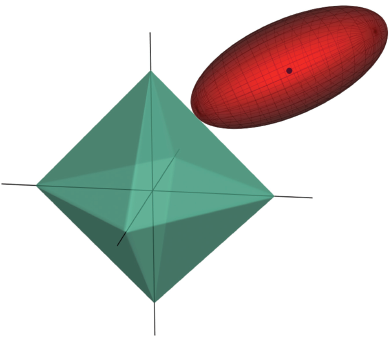
\includegraphics[width=0.7 \textwidth]{GLR2.png}\\[1cm] % Include a department/university logo - this will require the graphicx package
	 
	%----------------------------------------------------------------------------------------
	
	\vfill % Push the date up 1/4 of the remaining page
	
\end{titlepage}
\begin{abstract}
\textcolor{blue}{English} Lynhurtig Bradley-Terry modellen anvendes til at lave parvise sammenligninger af f.eks. fodboldhold styrker. i den oprindelig model (Bradley \& Terry 1952) antages at der altid vil være en vinder, men da dette er en urealistisk betragtning blev modellen udvidet (Rao-Kupper 1967). til at inkludere en grænseværdiparameter som gør det muligt at indrage udfaldet uafgjort. Dette papir tager udgangspunkt i denne model og betragter anvendelsen af LASSO optimering til udvælgelsen af parametre til estimering af de forskellige holds styrke. \textcolor{red}{Vi viser i denne opgave hvordan rao-kuppers model kan bruges til at rangere hold, og hvordan man ved tilføje et dynamisk element kan bruge den til at prædiktere udfald af parvise sammenligningen med tre udfald. Yderligere viser, hvordan lassostraf kan anvendes til at optimere denne prædiktion}
\end{abstract}
\clearpage
\renewcommand{\contentsname}{Indholdsfortegnelse}
\clearpage
\tableofcontents
\clearpage
\newpage
\pagenumbering{arabic}
\section{Indledning}
Indledning ...
\subsection{Problemformulering}
Problemformulering ...
\subsection{Afgrænsning}
Afgrænsning ...
\section{Generalisering af Bradley-Terry modellen}
I dette afsnit præsentere vi hvordan vi tolker Bradley-Terry modellen, hvordan vi bruger modellen til at lave parvise sammenligninger og hvordan vi estimere parametrene i modellen.\\\\
Bradley og Terry (1952)\cite{BradleyTerry} introducerer en statistisk model til at rangere f.eks. forbrugervurderinger af produkter eller styrker af fodboldhold ved parvise sammenligninger. Dette gøres ved at estimere nogle nytter for produkterne eller styrker af fodboldholdene. I førstnævnte eksempel vil modellen yderligere kunne bruges til at estimere sandsynligheden for, at en forbruger foretrækker ét produkt, over et andet - i sidstnævnte eksempel til at estimere sandsynligheden for, at BIF vinder over FCK i deres næste opgør.\\
\textcolor{blue}{Når vi i løbet af dette projekt beskriver forskellige modeller til parvise sammenligninger, vil vi altid tage udgangspunkt i sammenligningen af hold $i$ med hold $j$, hvor $i<j$ altid. Vi lader \\$i \in \{1,..,h-1\}$ og $j\in \{i+1,...,h\}$ hvor $h$ er antal produkter eller fodbold der sammenlignes. På denne måde undgår vi at gentage parvise sammenligninger af hold \textit{i} og hold \textit{j}, samt at sammenligne hold med sig selv}.  I dette projekt tager vi udgangspunkt i eksemplet med sammenligninger af fodboldhold. 
\subsection{Bradley-Terry modellen}
\sout{Når vi sammenligner hold \textit{i} med hold \textit{j}, betragter vi altid situationen $i<j$, hvor vi definerer \\$i \in \{1,..,h-1\}$ og $j\in \{i+1,...,h\}$ hvor $h\in \mathbb{Z}^+$ betegner antal hold. På denne måde undgår vi at gentage parvise sammenligninger mellem hold \textit{i} og hold \textit{j}, samt at sammenligne hold med sig selv.}\\
Vi skriver Bradley-Terry modellen \sout{sandsynligheden for at hold $i$ vinder over hold $j$}, som:
\begin{align*}
    P(i\ vinder\ over\ j) = p_{i\cdot ij} = \frac{\pi_i}{\pi_i+\pi_j},
\end{align*}
\textcolor{red}{$\pi_i>0?$}\\
hvor $p_{i\cdot ij}$ er sandsynligheden for at hold \textit{i} vinder over hold \textit{j}. Vi tolker $\pi_i$ og $\pi_j$ som hold \textit{i} og \textit{j}'s respektive styrker, og lader\sout{. Dermed kan }$Y_i=\pi_i+\epsilon_i$ betegne hold \textit{i}'s dagsform\sout{, hvor $\epsilon_i$ er fejlled.} Dette medfører hold \textit{i} vinder over hold \textit{j}, hvis $Y_i>Y_j$. 
\textcolor{blue}{Eftersom modellens parametre kan skaleres op uden at det påvirker sandsynlighederne;}
\begin{align*}
p_{i\cdot ij} = \frac{\pi_i}{\pi_i+\pi_j} = \frac{\pi_iC}{\pi_iC+\pi_jC},
\end{align*}
\textcolor{blue}{ ses modellen at være overparameteriseret}. \textcolor{blue}{Det er dermed ikke muligt, at} \sout{Vi kan dermed ikke} identificere de enkelte styrkeparametre, men \textcolor{blue}{det er muligt at}\sout{vi kan} identificere forholdet mellem to styrkeparametre. \textcolor{red}{Det problem klarer vi ved, at sætte et af holdenens styrker fast, eksempelvis hold $f$, for så at estimere de andre holds styrker relativt til hold $f$.}\sout{For at overkomme dette problem kan der lægges et bånd på, der sikrer, at vi kan estimere styrkeparametrene; dette kan gøres i form af $\pi_1 = 0$ eller $\sum_i^n \pi_i = 1$. }\\
Ved omskrivning af $p_{i\cdot ij}$ udtrykker vi dette styrkeforhold som:
\begin{align*}
    p_{i\cdot ij} &= \frac{\pi_i}{\pi_i+\pi_j}=\frac{1}{1+\frac{\pi_j}{\pi_i}}=\frac{1}{1+e^{-(\log(\pi_i)-\log(\pi_j))}}\\
    &=F(V_{i\cdot ij})=\int_{-\infty}^{V_{i\cdot ij}} \frac{\partial p_{i\cdot ij}}{\partial V_{i\cdot ij}} \text{ d}V=\frac{1}{1+e^{-V_{i\cdot ij}}},
\end{align*}
hvor $V_{i\cdot ij}=\log(\pi_i)-\log(\pi_j)$ beskriver log-styrken for hold \textit{i} i forhold til hold \textit{j}. \textcolor{blue}{Vi ser} \sout{Det ses altså} at sandsynligheden for at hold \textit{i} vinder over hold \textit{j} \textcolor{blue}{er bestemt ved forskellen i log-styrker for de to hold.}\sout{afhænger af forskellen i hold \textit{i} og hold \textit{j}'s styrker}. Eftersom 
\begin{align*}
&f(V_{i\cdot ij})=\frac{\partial p_{i\cdot ij}}{\partial V_{i\cdot ij}} = \frac{e^{-V_{i\cdot ij}}}{(e^{-V_{i\cdot ij}}+1)^2} \geq 0, \\ 
\intertext{samt at}
&\int_{-\infty}^\infty f(V_{i\cdot ij}) \text{  d} V_{i\cdot ij} = 1,
\end{align*}
er $f(V_{i\cdot ij})$ en tæthed for den logistiske fordeling, hvor $F(V_{i\cdot ij})$ er den tilhørende fordelingsfunktion, som for givne styrke parametre, kan opfattes som en sandsynlighed.\\
Sandsynligheden for at hold \textit{i} vinder over hold \textit{j} på en given kampdag, tolkes som sandsynligheden for at hold \textit{i}'s dagsform er bedre (større) end hold \textit{j}'s:
\begin{align*}
p_{i\cdot ij}&=P\big{\{}Y_i>Y_j\big{\}}
\\&=P\big{\{}(\pi_i-\pi_j)+(\epsilon_i-\epsilon_j)>0\big{\}}
\\&=P\big{\{}(\epsilon_i-\epsilon_j)>(\pi_j-\pi_i)\big{\}}
\\&=\frac{1}{1+e^{-(log(\pi_i)-log(\pi_j))}} 
\\&=\frac{\pi_i}{\pi_i+\pi_j}.\;\;
\end{align*}
\\
\textcolor{blue}{Vi antager, at $\epsilon_i$'erne være uafhængige og gumbel fordelte, fordi så er forskellen $\epsilon_i-\epsilon_j$ logistisk fordelt.}\sout{For at forskellene mellem fejlleddene $\epsilon_i-\epsilon_j$ er logistisk fordelt skal $\epsilon_i$'erne være uafhængige og gumbel fordelte.}
\subsection{Rao-Kupper modellen}
Indtil videre har vi antaget\sout{det været en antagelse} at en fodboldkamp altid har haft en vinder, men dette er ikke en realistisk antagelse, da fodboldkampe kan ende uafgjort. Det samme gælder forbrugervalget mellem to produkter. Realistisk set, kan en forbruger godt være ligeglad ved valget mellem to produkter, hvis produkterne giver forbrugeren \textcolor{red}{tilnærmelsesvist} den samme nytte. Rao og Kupper (1967) \cite{RaoKupper} foreslår en løsning på dette dilemma; at udvide Bradley-Terry modellen med en grænseværdiparameter $\theta$. $\theta$ betegner den forskel i dagsform der mindst skal være mellem to hold, for at der er en vinder; hvis $\|Y_i-Y_j\| < \theta$ bliver kampen uafgjort. Rao-Kupper opskrives som integralet af en tæthed ligesom Bradley-Terry, og giver sandsynlighederne:
\begin{equation}
\begin{split}
    p_{i\cdot ij}&=F(V_{i\cdot ij}-\eta)=\frac{\pi_i}{\pi_i+\theta \pi_j}\\
    p_{j\cdot ij}&=F(V_{j\cdot ij}-\eta)=1-F(V_{i\cdot ij}+\eta)=\frac{\pi_j}{\theta \pi_i+\pi_j}\\
    p_{0\cdot ij}&=F(V_{i\cdot ij}+\eta)-F(V_{i\cdot ij}-\eta)= \frac{\pi_i \pi_j(\theta^2 -1)}{(\pi_i+\theta \pi_j)(\theta \pi_i + \pi_j)} \label{Sandynligheder},
\end{split}
\end{equation}
hvor $\eta=\log(\theta)>0 \rightarrow\theta>1$ og $p_{0\cdot ij}$ er sandsynligheden for det nye udfald, uafgjort. Sandsynlighederne er direkte sammenlignelige med et rangeringssystem, hvor hvert udfald giver en forskellig rangering mellem de to hold. I fodbold får vinderholdet 3 point, taberholdet 0 point og hvis kampen ender uafgjort får begge hold 1 point. Ligeledes vil en forbruger der står overfor valget mellem to produkter, enten synes det ene produkt er bedre, dårligere eller lige så godt som det andet. \sout{De tre udfald er direkte sammenlignelige med et rangeringssytem,  da hvert af udfaldende ikke giver samme antal point; sejr = 3 point, uafgjort = 1 point og tab = 0 point. Ligeledes kan dette overføres til rangering af produktsammenligninger; bedre, ligeglad og dårligere.}
\subsection{Parameterestimering}
\textcolor{blue}{I dette afsnit viser vi en måde at estimere \textit{maximum likelihood} estimaterne og deres tilhørende fordeling for parametrene i Rao-Kupper modellen.
Rao-Kupper er en delmodel af den almindelige multinomialfordelingsmodel, som vi vil tage udgangspunkt i når vi opstiller likelihooden}.\\
Lad $y_{ij}(t)$ være en tredimensionel uafhængig stokastisk variabel, som repræsenterer en kamp mellem hold \textit{i} og hold \textit{j} til tidspunkt $t$. $y_{ij}(t)$'s, tilhørende udfaldsområde er dermed givet ved 0-1 variablene $\big{(}y_{i\cdot ij}(t),\;y_{j\cdot ij}(t),\;y_{0\cdot ij}(t)\big{)}$, som hhv. repræsenterer sejr til hold \textit{i}, sejr til hold \textit{j} og uafgjort: 
\begin{align*}
  y_{i\cdot ij}(t)&=\begin{cases}
1\text{, hvis hold $i$ vinder over hold $j$ til tidspunkt $t$}\\
0\text{, ellers}
\end{cases},\\
 y_{j\cdot ij}(t)&=\begin{cases}
1\text{, hvis hold $j$ vinder over hold $i$ til tidspunkt $t$}\\
0\text{, ellers}
\end{cases},\\
 y_{0\cdot ij}(t)&=\begin{cases}
1\text{, hvis hold $i$ og hold $j$ spiller uafgjort til tidspunkt $t$}\\
0\text{, ellers}
\end{cases},
\end{align*}
thi bliver de tilhørende sandsynligheder:
\begin{align*}
   &P\{y_{i\cdot ij}(t)=1\}=p_{i\cdot ij} &&P\{y_{j\cdot ij}(t)=1\}=p_{j\cdot ij} &&P\{y_{0\cdot ij}(t)=1\}=p_{0\cdot ij}.
\end{align*}
 Kontingenstabellen for kampe mellem hold $i$ og hold $j$ for en given periode $t=\{1,..,n\}$ kalder vi $Y_{ij}=(Y_{i\cdot ij},Y_{j\cdot ij},Y_{0\cdot ij})$, hvor:
\begin{align*}
    &Y_{i\cdot ij}=\sum_{t=1}^{n}y_{i\cdot ij}(t) &&Y_{j\cdot ij}=\sum_{t=1}^ny_{j\cdot ij}(t) &&Y_{0\cdot ij}=\sum_{t=1}^ny_{0\cdot ij}(t)
\end{align*}
\\
Yderligere lader vi $r_{ij}(t)$ være en 0-1 variabel som beskriver, hvorvidt hold $i$ har spillet mod hold $j$ til tidspunkt $t$:
\begin{align*}
r_{ij}(t)&=\begin{cases}
1\text{, hvis hold $i$ spiller mod hold $j$ til tidspunkt $t$}\\
0\text{, ellers}
\end{cases},
\end{align*}
og lader $R_{ij}=\sum_{t=1}^nr_{ij}(t)$ være antal kampe mellem hold $i$ og hold $j$ (gentagelser af $y_{ij}(t)$) for perioden $t=\{1,...,n\}$. \textcolor{blue}{$r_{ij}(t)$ og $R_{ij}$ er praktiske til at omskrive modellen, for at lette notationerne i udregningerne; $y_{0\cdot ij}(t)=r_{ij}(t)-y_{i\cdot ij}(t)-y_{j\cdot ij}(t)$ og $Y_{0\cdot ij}=R_{ij}-Y_{i\cdot ij}-Y_{j\cdot ij}$}
\sout{Til at estimere styrkeparametrene og $\theta$, vil vi gøre brug af maksimering af likelihooden, hvor likelihood-funktionen opstilles ved multinomialfordelingen med sandsynlighederne fra (\ref{Sandynligheder}). Likelihoodenfunktionen for Rao-Kupper modellen bliver:}
\textcolor{blue}{Likelihood-funktionen, som (Rao og Kupper 1967) foreslår skriver vi som:}
\begin{align}
\mathcal{L}\big{(}\pi_1,...,\pi_h,\theta\big{)} &= \prod_{i<j}p_{i\cdot ij}^{Y_{i\cdot ij}}p_{j\cdot ij}^{Y_{j\cdot ij}}p_{0\cdot ij}^{Y_{0\cdot ij}}  \nonumber\\
&= \prod_{i<j}\Big{(}\frac{\pi_i}{\pi_i+\theta\pi_j}\Big{)}^{Y_{i\cdot ij}} \label{func:LikelihoodUdenBeta}
\;\Big{(}\frac{\pi_j}{\pi_j+\theta\pi_i}\Big{)}^{Y_{j\cdot ij}}
\Big{(}\frac{(\theta^2-1)\pi_i \pi_j}{(\pi_i+\theta\pi_j)(\pi_j+\theta\pi_i)}\Big{)}^{Y_{0\cdot ij}}\\
&=\prod_{i<j}\Big{(}\frac{\pi_i}{\pi_i+\theta\pi_j}\Big{)}^{Y_{i\cdot ij}}
\;\Big{(}\frac{\pi_j}{\pi_j+\theta\pi_i}\Big{)}^{Y_{j\cdot ij}}
\Big{(}\frac{(\theta^2-1)\pi_i  \pi_j}{(\pi_i+\theta\pi_j)(\pi_j+\theta\pi_i)}\Big{)}^{R_{ij}-{Y_{i\cdot ij}}-{Y_{j\cdot ij}}},\nonumber\\ \nonumber
\end{align}
hvor multinomialkoefficienten er udeladt, da den ligegyldig når vi estimere parametre. Her bliver likelihooden opstillet i forhold til antal sejr, tabte og uafgjorte mellem hver parvis sammenligning for en periode.\textcolor{blue}{ En anden mulighed er at opskrive modellen, hvor i stedet for at kontingenstabellen indeholder udfald for hele perioden, så opdaterer den løbende for hvert tidspunkt i perioden. I denne dynamiske version af Rao-Kupper modellen bliver likelihooden:}
\begin{align*}
\mathcal{L}\big{(}\pi_1,...,\pi_h,\theta\big{)}
&=\prod_t\prod_{i<j}\Big{(}\frac{\pi_i}{\pi_i+\theta\pi_j}\Big{)}^{y_{i\cdot ij}(t)}
\;\Big{(}\frac{\pi_j}{\pi_j+\theta\pi_i}\Big{)}^{y_{j\cdot ij}(t)}
\Big{(}\frac{(\theta^2-1)\pi_i \pi_j}{(\pi_i+\theta\pi_j)(\pi_j+\theta\pi_i)}\Big{)}^{y_{ij}(t)-{y_{i\cdot ij}(t)}-{y_{j\cdot ij}(t)}}.
\end{align*}
Her giver vi modellen et dynamisk aspekt, hvor det blandt andet er muligt at inkludere kampspecifikke kovariater. Vi kommer mere ind på forskellen mellem Rao-Kupper modellen og dens dynamiske version når vi implementere dem. \textcolor{blue}{Parametrene bliver estimeret med samme metoder og i resten af afsnittet tager vi udgangspunkt i Rao-Kupper modellen.} 
Først opskriver vi log-likelihooden: 
\textcolor{blue}{Det vil være fint allerede her, at omskrive den som ved første ordens betingelserne..}
\begin{align*}
\textit{l}(\pi,\theta)
&=\sum_{i<j}\Big{[}Y_{i\cdot ij}\log\Big{(}\frac{\pi_i}{\pi_i+\theta\pi_j}\Big{)}
+ Y_{j\cdot ij}\log\Big{(}\frac{\pi_j}{\pi_j+\theta\pi_i}\Big{)}\\
&+ (R_{ij}-Y_{i\cdot ij}-Y_{j\cdot ij}) \log\Big{(}\frac{(\theta^2-1)\pi_i \pi_j}{(\pi_i+\theta\pi_j)(\pi_j+\theta\pi_i)}\Big{)}\Big{]}
\end{align*}
\#\textcolor{blue}{Vi vælger, at omskrive styrkerne til $\pi_i=e^{\gamma_i}$, hvor $\gamma_i=\log(pi_i)$, for at fjerne den nedre grænse $\pi_1\geq0$:} \sout{Som log-likelihooden ser ud i ovenstående, er der ikke noget der hindrer negative styrker. Dog er det klart at et forhold mellem en negativ styrke og en positiv styrke vil være misvisende, hvorfor vi log-transformerer styrkerne ved at sætte $\gamma_i=\log(\pi_i)$ og $\gamma_j=\log(\pi_j)$:}\\
\begin{align*}
\textit{l}(\gamma,\theta)
&=\sum_{i<j}\Big{[}Y_{i\cdot ij}\Big{(}\gamma_i-\log(e^{\gamma_i}+\theta e^{\gamma_j})\Big{)}
+Y_{j\cdot ij}\Big{(}\gamma_j-\log(e^{\gamma_j}+\theta e^{\gamma_i})\Big{)}\\
& +(r_{ij}-Y_{i\cdot ij}-Y_{j\cdot ij}) \Big{(} \log(\theta^2-1)+\gamma_i+\gamma_j-\log(e^{\gamma_i}+\theta e^{\gamma_j})-\log(e^{\gamma_j}+\theta e^{\gamma_i})\Big{)}.
\end{align*}
\textcolor{blue}{Vi sætter nu $\gamma_i=x_i^T\beta$, hvor $x_i$ er den $i$'te række i designmatricen, som indeholder observationer for hold $i$ og $\beta$ er den tilhørende parametervektor. MÅSKE FORKLAR SØJLERNE:}
\sout{Til at implementere dette forhold i log-likelihooden, som vi skal maksimere ud fra parametrerne, indsætter vi $\gamma_i=x_i^T\beta$ og $\gamma_j=x_j^T\beta$:}\\
\begin{align*}
   \sout{ p_{i\cdot ij} = \frac{1}{1+ e^{-(log(\pi_i)-log(\pi_j))}} = \frac{1}{1+ e^{-\beta(x_i^T-x_j^T)}},}
\end{align*}
hvor $x_i$ er den i'te søjle i designmatricen og $\beta$ er vores parametervektor. Designmatricens \textit{i}'te søjle indeholder altså data for hold \textit{i}, hvor den \textit{k}'te række indeholder data til den \textit{k}'te parameter i parametervektoren $\beta$. \\
I vores tilfælde vil det være data der beskriver to fodboldhold, men formen vil forblive uændret hvis det er to forbrugerprodukter der bliver sammenlignet.
\begin{align*}
\textit{l}(\beta,\theta)
&=\sum_{i<j}\Big{[}Y_{i\cdot ij}\Big{(}x_i^T\beta-\log(e^{x_i^T\beta}+\theta e^{x_j^T\beta})\Big{)}
+Y_{j\cdot ij}\Big{(}x_j^T\beta-\log(e^{x_j^T\beta}+\theta e^{x_i^T\beta})\Big{)}\\
& +(r_{ij}-Y_{i\cdot ij}-Y_{j\cdot ij}) \Big{(} \log(\theta^2-1)+x_i^T\beta+x_j^T\beta-\log(e^{x_i^T\beta}+\theta e^{x_j^T\beta})-\log(e^{x_j^T\beta}+\theta e^{x_i^T\beta})\Big{)}\Big{]}.
\end{align*}
\textcolor{blue}{Til at estimere vores parametre vælger vi, at benytte den iterative Newton-Rhapson algoritme:}\sout{For at bestemme maksimum-likelihood estimaterne for vores parametre, har vi valgt at gøre brug af den iterative metode, Newton-Raphson. Newton-Raphson opstilles på følgende form, med den observerede information og scorefunktionen:}
\begin{align*}
v_{c+1} = v_{c} + i(v_{c})^{-1}s(v_{c})\omega,
\end{align*}
hvor $v_{c}=\begin{bmatrix} \beta\\\theta\end{bmatrix}$ er en vektor som indeholder parametrene $\beta$ og $\theta$. $s(v_{c})$ er scorefunktionen som afgøre retningen af hver iteration, $i(v_c)$ er den observerede information som afgører længden af skridtet og $\omega$ er en \textcolor{red}{korrigering} af skridtlængden. \sout{ bestående af vores styrkeparametre, $\pi_i$, samt $\theta$ parametre ($\beta$ og $\theta$) og $\omega$ er skridtlængden. Eftersom parvise sammenligninger i praksis, afhænger af den data der er indsamlet, vil det være nødvendigt at have et udtryk for likelihooden i form af den data der er indsamlet. For at gøre dette, definerer vi et udtryk for samtlige $\log( \pi_i)$'er (også for referencegruppen). Dette indses ved indsættelse i den lineære sammenhæng mellem styrkerne:}

Førsteordensbetingelserne for $\beta$ og $\theta$ bliver:
\begin{align*}
\frac{\partial \ell(\beta;\theta)}{\partial \beta}&= 
\sum_{i<j}\Big{[}\Big{(}
(R_{ij}-Y_{i\cdot ij})\Big{(}-\frac{\theta e^{x_i^T\beta}}{e^{x_j^T\beta}+\theta e^{x_i^T\beta}}\Big{)}+(R_{ij}-Y_{j\cdot ij})\Big{(}\frac{\theta e^{x_j^T\beta}}{e^{x_i^T\beta}+\theta e^{x_j^T\beta}}\Big{)}\Big{)}(x_i-x_j)\Big{]},\\
\frac{\partial \ell(\beta;\theta)}{\partial \theta}&=
\sum_{i<j}
\Big{[}
 (R_{ij}-Y_{i\cdot ij}-Y_{j\cdot ij})\Big{(}\frac{2\theta}{\theta^2-1}\Big{)}\\
 &+(R_{ij}-Y_{i\cdot ij})\Big{(}-\frac{e^{x_i^T\beta}}{\theta e^{x_i^T\beta}+e^{x_j^T\beta}}\Big{)}
 +(R_{ij}-Y_{j\cdot ij})\Big{(}-\frac{e^{x_j^T\beta}}{e^{x_i^T\beta}+\theta e^{x_j^T\beta}}\Big{)}
\Big{]},\\
\end{align*}
Dermed bliver scorefunktionen:
\begin{equation}
s\big{(}\beta,\theta\big{)} = \begin{bmatrix}
\frac{\partial \ell(\beta;\theta)}{\partial \beta}\\
\frac{\partial \ell(\beta;\theta)}{\partial \theta}
\end{bmatrix},
\label{score}
\end{equation}
hvor førsteordensbetingelsen med hensyn til $\beta$ bliver en vektor med længde lig antal \sout{rækker} søjler i designmatricen. 
\sout{Udledningerne til}. Andensordsbetingelserne bliver ligeledes: 
\begin{align}
\frac{\partial^2 \ell(\beta;\theta)}{\partial \beta^2}
&= \sum_{i<j}\Big{[}\Big{(} -\frac{(R_{ij}-Y_{i\cdot ij})}{(\theta e^{x_i^T\beta}+e^{x_j^T\beta})^2}-\frac{(R_{ij}-Y_{j\cdot ij})}{(e^{x_i^T\beta}+\theta e^{x_j^T\beta})^2}\Big{)}e^{x_i^T\beta+x_j^T\beta}\theta\big{(}x_{i}-x_{j}\big{)}\big{(}x_{i}-x_{j}\big{)}^T\Big{]},\label{func:d2db2}\\
\frac{\partial^2 \ell(\beta;\theta)}{\partial \theta^2}
&= \sum_{i<j} 
\Big{[}
(R_{ij}-Y_{i\cdot ij}-Y_{j\cdot ij})\Big{(}-\frac{2(\theta^2+1)}{(\theta^2-1)^2}\Big{)}\\ \nonumber
&+(R_{ij}-Y_{i\cdot ij})\Big{(}\frac{e^{2x_i^T\beta}}{(\theta e^{x_i^T\beta}+e^{x_j^T\beta})^2}\Big{)}
+(R_{ij}-Y_{j\cdot ij})\Big{(}\frac{e^{2x_j^T\beta}}{(e^{x_i^T\beta}+\theta e^{x_j^T\beta})^2}\Big{)}\Big{]},\label{func:d2dt2}\\
\frac{\partial^2 \ell(\beta;\theta)}{\partial \beta\partial \theta}
&= \sum_{i<j}\Big{[}\Big{(}
-\frac{(R_{ij}-Y_{i \cdot ij})}{(\theta e^{x_i^T\beta}+e^{x_j^T\beta})^2}
+\frac{(R_{ij}-Y_{j \cdot ij})}{(e^{x_i^T\beta}+\theta e^{x_j^T\beta})^2}\Big{)}e^{x_i\beta+x_j\beta}(x_{i}-x_{j})\Big{]},\label{func:d2dbt}
\end{align}
\sout{hvorved vi nu får at andenordensbetingelsen ift. $\beta$ bliver en kvadratisk matrice, hvorfor den observerede informationen opskrives som en symmetrisk blok-matrix på formen:}
hvorved vi opskriver den observerede information som den symetriske blok-matrice:
\begin{align*}
i(\beta,\theta) = -\begin{bmatrix}
\frac{\partial^2 \ell(\beta;\theta)}{\partial \beta^2} &\frac{\partial^2 \ell(\beta;\theta)}{\partial \beta \partial \theta} \\
\Big{(}\frac{\partial^2 \ell(\beta;\theta)}{\partial \beta \partial \theta}\Big{)}^T & \frac{\partial^2 \ell(\beta;\theta)}{\partial \theta^2}
\end{bmatrix},
\label{inf}
\end{align*}
Hvor den anden afledte med hensyn til $\beta$ er en $k\times k$ matrice, den anden afledte med hensyn til $\theta$ er $1 \times 1$ og de anden afledte med hensyn til $\beta$ og $\theta$ er vektorer med længde $k$. 
\sout{Likelihooden konvergerer mod et maksimum givet scorefunktionen (\ref{score}) og den observerede information (\ref{inf}), hvis den observerede information (\ref{inf}) er positiv semi-definit.} For at sikrer, at Newton-Rhapson konvergerer mod et globalt maksima, kræver det at vores likelihood funktion er konkav; hvilket er tilfældet, hvis den observerede information er \textit{positivt semi-definit} (PSD). \sout{$i(\beta,\theta)$ er symmetrisk kan vi benytte}. Vi benytter Albert (1972)\cite{Albert}'s sætning til at tjekke, hvorvidt en symmetrisk blok-matrice er PSD:  \\\textbf{ Alberts sætning} \textit{Lad M være en symmetrisk blok-matrice, så:}
\begin{align*}
&M = \begin{bmatrix}
A & B\\
C & D
\end{bmatrix}\geq 0 \iff \\
&(i)\; D\geq0\\
&(ii)\; C=D^{-1}DC\\
&(iii)\; A\geq BD^{-1}C\\
\end{align*}  
ad (\textit{i}) ønsker vi, at vise: 
\begin{align*}
&-\frac{\partial^2 \ell(\beta;\theta)}{\partial \theta^2} \geq 0 \iff &(R_{ij}- Y_{i\cdot ij}-Y_{j\cdot ij}) \frac{2(\theta^2+1)}{(\theta^2-1)^2} \geq (R_{ij}-Y_{i\cdot ij})p_{i\cdot ij}^2 + (r_{ij}-Y_{j\cdot ij})p_{j\cdot ij}^2
\end{align*}. Vi antager, at der altid er mindst et udfald som er uafgjort/ giver samme nytte, fordi ellers vil udvidelse til Rao-Kupper modellen være overflødig.\sout{Det antages, at vi har mindst én uafgjort kamp i det datasæt vi undersøger, }$(R_{ij}- Y_{i\cdot ij}-Y_{j\cdot ij}) > 0$.
\\Observation I: Vi ser, at når antal af uafgjorte går mod 0, konvergerer $\theta$ mod 1, hvilket medfører venstre siden i uligheden bliver \sout{numerisk} stor. $p_{i\cdot ij}^2$ og $p_{j\cdot ij}^2$ vil også blive store, men de to kvadrerede sandsynligheder vil stadig have en sum mindre end 1.\\
Observation II: Derudover ser vi, at når antallet af uafgjorte går mod $\infty$, vil $\theta$ gå mod $\infty$ og $Y_{i \cdot ij} \text{ og } Y_{j \cdot ij}$ gå mod 0. Det betyder at både højresiden og venstre siden konvergerer mod 0.\sout{bliver stort er meget stor vil både venstre og højre side konvergere mod 0. Dette ses for venstresiden da $\theta$ går mod  $\infty$, og for højresiden da sandsynlighederne for sejr til hold $i$ og $j$ går mod 0.} Hvilken af dem der konvergere hurtigst kan ikke siges uden konkrete observationer for $Y$'erne. I vores eksempel med fodbold kampe vil tilfældet, hvor antal uafgjorte går mod et tal som er langt større end antal sejrer og tabte tilsammen være yderst sjældent, hvis stikprøven er stor nok \textcolor{red}{- nok aldrig set i fodboldens historie}. \textcolor{blue}{Hvis modellen istedet skulle testes på eksempelvis blind smagning af pilsner-øl, er forventningerne sandsynligvis anderledes.}\sout{Dog vil tilfældet hvor $Y_{0 \cdot ij}$ er større end $Y_{i \cdot ij} \text{ og } Y_{j \cdot ij}$ for mange hold, være yderst sjældent da udfaldet uafgjort ikke fremkommer så hyppigt, som de andre to tilsammen.}\\
ad (\textit{ii}) ønsker vi, at vise:
\begin{align*}
\Big{[}-\frac{\partial^2 \ell(\beta,\theta)}{\partial \beta \partial \theta}\Big{]}^T = \Big{[}-\frac{\partial^2 \ell(\beta;\theta)}{\partial \theta^2}\Big{]}^{-1}\Big{[}-\frac{\partial^2 \ell(\beta;\theta)}{\partial \theta^2}\Big{]}\Big{[}-\frac{\partial^2 \ell(\beta,\theta)}{\partial \beta \partial \theta}\Big{]}^T
\end{align*}
Vi ved, at den andenafledte med hensyn til $\theta$ er endimensionel og derfor er invertibel så længde den er forskellig fra 0. Det vil sige, at så længe $(i)$ gælder med streng ulighed er $\Big{[}-\frac{\partial^2 \ell(\beta;\theta)}{\partial \theta^2}\Big{]}^{-1}\Big{[}-\frac{\partial^2 \ell(\beta;\theta)}{\partial \theta^2}\Big{]}=1$, så ligningen er opfyldt.\\
ad (\textit{iii}) ønsker vi, at vise:
\begin{align*}
  \Big{[}-\frac{\partial^2 \ell(\beta;\theta)}{\partial \beta^2}\Big{]} \geq \Big{[}-\frac{\partial^2 \ell(\beta;\theta)}{\partial \beta \partial \theta}\Big{]}\Big{[}-\frac{\partial^2 \ell(\beta;\theta)}{\partial \theta^2}\Big{]}\Big{[}-\frac{\partial^2 \ell(\beta;\theta)}{\partial \beta \partial \theta}\Big{]}^T
\end{align*}
Vi ser fra fra ligning (\ref{func:d2db2}), at $-\frac{\partial^2 \ell(\beta;\theta)}{\partial \beta^2}$, er på formen: $C_1(x_i-x_j)(x_i-x_j)^T$ hvor $C_1$ er en positiv konstant, og er derfor større end 0. \textcolor{red}{Det ved vi fra sylvesters kriterie tror jeg}
Vi ser fra ligning (\ref{func:d2dbt}) at $\big{[}\frac{\partial^2 \ell(\beta;\theta)}{\partial \beta \partial \theta}\big{]}\big{[}\frac{\partial^2 \ell(\beta;\theta)}{\partial \beta \partial \theta}\big{]}^T$, skrives på formen $C_2^2(x_i-x_j)(x_i-x_j)^T$ og er derfor også større end nul. \textcolor{blue}{ Den inverse af den andenafledte med hensyn til $\theta$ bliver en positiv skalar, hvis $(i)$ holder.} Størrelserne på $C_1$ og $C_2$ afhænger fordeling af udfald, hvor $C_1$ ændres i forhold til $R_{ij}-Y_{i\cdot ij} + R_{ij}-Y_{j\cdot ij}$ og $C_2$ ændres i forhold til $R_{ij}-Y_{i\cdot ij} - R_{ij}-Y_{j\cdot ij}$. Hvis der er mange uafgjorte kampe vil $C_1$ blive stor relativt til $C_2^2$. $C_2^2$ vil gå mod 0 og ligeledes blive lille relativt til $C_1$, hvis antallet af sejrer for hold $i$ og hold $j$ går mod hinanden. Hvis derimod forskellen i sejrer for hold $i$ og hold $j$ bliver stor, vil $C_2^2$ bliver stor i forhold til $C_1$. \sout{ Derudover har vi at $BD^{-1}C$ også er positiv, da $D^{-1}>0$ eftersom $D$ i vores tilfælde er endimensionelt, samt at eftersom $B$ og $C$ altid vil have samme fortegn, vil deres produkt være positivt.} Hvorvidt $(iii)$ er opfyldt, vil derfor i høj grad komme an på fordelingen af $Y$'erne. \\\\
Konklusion er, at vores observerede information formentligt er PSD på et stort område. \sout{for samtlige $\theta$'er. Hvorimod $\beta$'erne for et låst $\theta$, vil konvergere, da $A$ altid er positiv.}\\
For at sikrer os, at vi befinder os på en konkav mængde i likelihood funktionen, vælger vi tilføje et tjek i vores Newton-Rhapson algoritme, for hvorvidt Alberts sætning er opfyldt. \\
\textcolor{red}{ER ALT DET MED PROFIL LIKELIHOOD RELEVANT, VI GØR DET IKKE?\\
1) Finde Profillikelihooden for $\beta$'erne, hvor $\theta$ holdes fast.\\
2) Sætte initialiseringsværdierne til at være inde i mængden, og derefter foretage et skridt der forbliver i mængden. Til at finde en skridtlængde der opfylder Alberts sætning vil vi gøre brug af \textit{linesearch}, som foreslået af Kevin P. Murphy (2012) \cite{LineSearch}. Denne metode sikrer sig at likelihooden konvergerer (når den er i mængden der opfylder Alberts sætning), samtidig med at den forøger likelihooden mest muligt for hvert skridt. Dette gøres altså i hvert skridt i Newton-Raphson, hvor vi finder en skridtlængde, $\omega$, der opfylder:}\\
\begin{align*}
    v_{c+1} &= v_{c} -  i(\beta_c,\theta_c)^{-1}s(\beta_c,\theta_c)\omega,\\
    \ell(v_{c}) &< \ell(v_{c+1}),
\end{align*}
hvor vi tester skridtlængderne i faldende orden, og $\omega$ vælges for det første tilfælde der opfylder betingelsen $\ell(v_c)<\ell(v_{c+1})$. 
Her kan problemet opskrives som 
$\max_{\omega \in \mathcal{N}} \ell(v_{c+1})$, hvor vi i vores tilfælde vælger 
$\mathcal{N} = \{1,\frac{1}{2},...,\frac{1}{100}\}$. Ulempen ved denne metode er at det kan være tungt at udregne likelihooden, og dermed være tungt at finde en skridtlængde; især hvis den skridtlængde der øger likelihooden er lille. På den anden side, så sørger denne metode for at man får den størst mulige skridtlængde, og hvis alternativet er at vælge en lav skridtlængde hver gang (for at sikre sig at man øger likelihooden hver gang), så kan denne metode øge konvergeringshastigheden.\\
I praksis vil tiltag 2) være mere medgørlig at implementere, eftersom 1) vil kræve markant flere iterationer, da der først skal itereres over $\beta$'erne og derefter over $\theta$. En metode til at finde profillikelihooden i praksis er at udføre Newton-Raphson hvor $\theta$ holdes fast, og $\theta$ ændres hvis den ikke kan konvergere hvorefter der prøves igen for den nye $\theta$.\par
Standardfejlene for vores estimerede parametre, $\beta$ og $\theta$ finder vi ud fra kovariansmatricen ($\hat{\Sigma}$): 
\begin{align*}
&\hat{\sigma}^2_{\beta,\theta}=i(\beta,\theta)^{-1}=
\Big{(}-\begin{bmatrix}
\frac{\partial^2 \ell(\beta;\theta)}{\partial \beta^2} &\frac{\partial^2 \ell(\beta;\theta)}{\partial \beta \partial \theta} \\
\Big{(}\frac{\partial^2 \ell(\beta;\theta)}{\partial \beta \partial \theta}\Big{)}^T & \frac{\partial \ell(\beta;\theta)}{\partial \theta^2}
\end{bmatrix}\Big{)}^{-1}\\
\end{align*}
\begin{align}
\intertext{Standardfejlene $\hat{\sigma}_\beta$ og $\hat{\sigma}_\theta$ findes ved kvadratroden af diagonalen af $\hat{\sigma}^2_{\beta,\theta}$}
\hat{\sigma}_{\beta,\theta}=\sqrt{\text{diag}(\hat{\sigma}^2_{\beta,\theta})}=
\begin{bmatrix}
\hat{\sigma}_{\beta_1}& &\\
& \ddots & \\
& & \hat{\sigma}_{\beta_k} \\
& & & \hat{\sigma}_{\theta}
\end{bmatrix}
\end{align}
Vi estimere den approksimative fordeling af styrkerne med delta-metoden. Når vi estimere styrkerne gør vi det relativt til ét af holdene, hold $i$ relativt til hold $h$ betyder at $x_i\Rightarrow x_i-x_h$.
\begin{align*}
\intertext{Først beregner vi variansen på $\log(\hat{\pi}_i)=x_i^T\hat{\beta}$}
\text{Var}\big{[}\log(\hat{\pi}_i)\big{]}
&=\frac{\partial x_i^T\beta}{\partial\beta}\hat{\sigma}^2_{\beta}\frac{\partial x_i^T\beta}{\partial \beta}=x_i^T\hat{\sigma}^2_\beta x_i,\\
\intertext{hvor $\hat{\sigma}^2_{\beta}$ er lig $\hat{\sigma}^2_{\beta,\theta}$ uden sidste række og søjle. Ved delta-metoden fås variansen på $\hat{\pi}_i=e^{x_i^T\hat{\beta}}$:}
\text{Var}\big{[}\hat{\pi}_i\big{]}&=\frac{\partial e^{(x_i^T\hat{\beta})}}{\partial(x_i^T\hat{\beta})}\text{Var}\big{[}\log(\hat{\pi}_i)\big{]}\frac{\partial e^{(x_i^T\hat{\beta})}}{\partial(x_i^T\hat{\beta})}=e^{(x_i^T\hat{\beta})}\big{(}x_i^T\hat{\sigma}^2_\beta x_i\big{)}e^{(x_i^T\hat{\beta})},\\
\intertext{thi bliver standardfejlen på $\hat{\pi}_i$}
\hat{\sigma}_{\pi_i}&=\sqrt{\text{Var}\big{[}\hat{\pi}_i\big{]}}=\sqrt{e^{(x_i^T\hat{\beta})}\big{(}x_i^T\hat{\sigma}^2_\beta x_i\big{)}e^{(x_i^T\hat{\beta})}}.\\
\intertext{Den approksimative fordeling af styrkerne bliver:}
\hat{\pi_i} & \sim N\Big{(}e^{(x_i^T\beta)},e^{(x_i^T\hat{\beta})}\big{(}x_i^T\hat{\sigma}^2_\beta x_i\big{)}e^{(x_i^T\hat{\beta})}\Big{)}
\intertext{Senere vil vi sammenligne Rao-Kupper modellen med en dynamiske version af modellen. I den dynamiske model beregnes styrken for et hold som et gennemsnit af holdets styrker udregnet på forskellige tidspunkter. Vi kalder gennemsnits styrken for hold $i$ til tidspunkt t for $\overline{\hat{\pi}_i}(t)=\frac{1}{t}\big{(}e^{x_i^T(1)\hat{\beta}}+...+e^{x_i^T(t)\hat{\beta}}\big{)}$. Variansen på $\overline{\hat{\pi}_i}(t)$ bliver:}
\text{Var}\Big{[}\overline{\hat{\pi}_i}(t)\Big{]}&=\text{Var}\big{[}\overline{e^{\big{(}x_i^T(t)\hat{\beta}\big{)}}}\big{]}=\overline{e^{\big{(}x_i^T(t)\hat{\beta}\big{)}}}\big{(}\overline{x_i}^T\hat{\sigma}^2_\beta\overline{x_i}\big{)}\overline{e^{\big{(}x_i^T(t)\hat{\beta}\big{)}}},\\
\intertext{thi bliver standardfejlen på $\overline{\hat{\pi}_i}(t)$:}
\hat{\sigma}_{\overline{\pi_i}}&=\sqrt{\overline{e^{\big{(}x_i^T(t)\hat{\beta}\big{)}}}\big{(}\overline{x_i}^T\hat{\sigma}^2_\beta\overline{x_i}\big{)}\overline{e^{\big{(}x_i^T(t)\hat{\beta}\big{)}}}},
\intertext{og den approksimative fordeling af styrkerne i den dynamiske model bliver:}
\overline{\hat{\pi_i}}(t) & \sim N\Big{(}\;\overline{e^{(x_i^T(t)\beta)}},\overline{e^{\big{(}x_i^T(t)\hat{\beta}\big{)}}}\big{(}\overline{x_i}^T\hat{\sigma}^2_\beta\overline{x_i}\big{)}\overline{e^{\big{(}x_i^T(t)\hat{\beta}\big{)}}}\;\Big{)}
\end{align*}

\subsection{Hypotesetest af modellen}
I dette afsnit viser vi, hvordan vi evaluere vores model ud fra et givent datasæt i praksis, hvor det er antaget at det valgte datasæt er komplet, repræsentativt og stort. \par
På trods af at dataet er valgt ud fra forventningen om, at de beskrivende variable afspejler de observerede udfald, er dette ikke altid gældende. Til at teste, hvorvidt variablene beskriver de observerede udfald udføre vi en kvotienttest, med nulhypotesen:\\
$H_0: \hat{\beta} = 0$\\
Hvis der ikke er evidens for at $\hat{\beta}$'erne er forskellige fra 0, betyder det i vores tilfælde med fodbold, at holdenes styrker ikke har nogen indflydelse på udfaldene (da alle styrkerne vil blive ens). Vores kovtientest bliver:
\begin{align*}
\textcolor{blue}{Q} LR = -2\Big{(}\text{max}_\theta \;\ell (\beta_{H_0},\theta)-\ell (\beta_{MLE},\theta_{MLE})\Big{)},
\end{align*}
hvor teststørrelsen maksimeres ift. $\theta$ med $\hat{\beta}$ holdt fast lig 0. Her antages det, at for store stikprøver, er LR omtrent $\chi^2$-fordelt med $(k-1)$ frihedsgrader. \\
Vi undlader at teste for om $\theta=1$, da Rao-Kupper udvidelsen dermed bliver nyttesløs, eftersom udfaldet uafgjort vil være udeladt fra modellen. \par
Derudover er det nyttigt at kigge på residualerne, for at tjekke om der er en sammenhæng mellem de fittede værdier og deres tilhørende residualer. De rå residualer for kampene mellem hold $i$ og hold $j$ i Rao-Kupper modellen bliver:
%Modellen kan i sin helhed testes ved en $\chi^2$ Goodness of Fit test, hvor vi kan teste de kumulerede sandsynligheder op imod de observerede sandsynligheder fra kontingenstabellen. Vi kan opstille en kontingenstabel for de forventede udfald ud fra $\hat{Y}_{ij}(t) = (p_{i\cdot ij},p_{j\cdot ij},p_{0\cdot ij})$, som er udregnet ved brug af de estimerede $\hat{\beta}$ og $\hat{\theta}$:
%For at tjekke modellen igennem er det praktisk udregne residualerne:
\begin{align*}
&\epsilon_{i\cdot ij}=Y_{i\cdot ij}-R_{ij}\hat{p}_{i\cdot ij}
&&\epsilon_{j\cdot ij}=Y_{i\cdot ij}-R_{ij} \hat{p}_{j\cdot ij}
&&\epsilon_{0\cdot ij}=Y_{0\cdot ij}-R_{ij} \hat{p}_{0\cdot ij}
\end{align*}
%\begin{align*}
%&\hat{Y}_{i\cdot ij} = r_{ij}\frac{e^{x_i^T\beta}}{e^{x_i^T\beta}+\theta e^{x_j^T\beta}},
%&&\hat{Y}_{j\cdot ij} = r_{ij}\frac{e^{x_j^T\beta}}{e^{x_j^T\beta}+\theta e^{x_i^T\beta}},
%&&\hat{Y}_{0\cdot ij} = r_{ij}\frac{(\theta^2-1)e^{x_i^T\beta}e^{x_j^T\beta}}{(e^{x_i^T\beta}+\theta e^{x_j^T\beta})(e^{x_i^T\beta}\theta +e^{x_j^T\beta})}.
%\end{align*}
%Vores $\chi^2$ teststørrelse bliver:
%\begin{align*}
%\chi^2 = \sum_{i<j} \frac{(Y_{i\cdot ij}-\hat{Y}_{i\cdot ij})^2}{\hat{Y}_{i\cdot ij}} + \frac{(Y_{j\cdot ij}-\hat{Y}_{j\cdot ij})^2}{\hat{Y}_{j\cdot ij}} + \frac{(Y_{0\cdot ij}-\hat{Y}_{0\cdot ij})^2}{\hat{Y}_{0\cdot ij}}
%\end{align*}
%Her vil det også gælde for tilstrækkeligt store stikprøver at teststørrelsen er $\chi^2$ fordelt, og her med $(h^2-2h)$ frihedsgrader. \\
\section{Modelovervejelser og data}
I dette afsnit viser vi hvordan vi anvender Rao-Kupper modellen i praksis. Vi stiller modellen op på to forskellige måder og tester dem begge i at rangere fodbold hold i den danske superliga for en sæson. 
\subsection{Implementering af modellen}
Når det kommer til implementering af Rao-Kupper, er det først og fremmest vigtigt at afklare hvad formålet med modelleringen er. Vi har valgt at stille modellen op på to forskellige måder. Den første er modellen som Rao og Kupper (1967)\cite{RaoKupper} præsentere den, hvor kovariaterne er faste over tid. I vores eksempel med fodbold betyder det, at holdenes styrker er faste over tid, så sandsynligheden for at hold $i$ vinder over hold $j$ er den samme for et hvilket som helst tidspunkt.
\sout{, hvor styrkerne er faste over tid, hvis formål er at rangere en gruppe af eksempelvis fodboldhold, efter respektive styrker for en given periode. Her er styrkerne udregnet ved gennemsnit af præstationer for perioden. Det var denne model (Rao og Kupper 1967) foreslog.} 
Den anden er en dynamisk version af modellen, hvor kovariaterne ændrer sig over tid. Dermed ændrer styrkerne og således sandsynlighederne sig fra kamp til kamp. \textcolor{blue}{Vores forventning er, at når vi ønsker at rangere en række fodboldhold, eller eventuelt en række produkter for en given periode, vil det være optimalt at benytte modellen som Rao og Kupper præsentere den, \textcolor{red}{hvor vi ser på perioden som helhed.} Men når vi ønsker at forudsige udfaldet af en fodboldkamp, eller en forbrugers foretruknevalg ved sammenligning af to produkter på et givent tidspunkt, vil der være en fordel i at bruge den dynamiske model. Det skyldes, at vi en den dynamiske model med kovariater der ændrer sig over tid har mulighed for at inkludere kamp/tidspunkts specifikke variable, som eksempelvis hjemmebanefordel eller vejr, samt sørge for, at en kamp på et givent tidspunkt kun bliver beskrevet af observationer fra tidligere tidspunkter (tidligere kampe) - dvs. sikrer os, at udfaldet af en fodbold kamp ikke blive beskrevet af observationer fra kampen selv.}
\sout{Denne models formål er at estimere sandsynlighederne for udfaldet af en kamp mellem to hold på et givet tidspunkt.} I vores eksempel med fodbold vil et tidspunkt være en spillerunde. En fodboldsæson bliver delt op i spillerunder, hvor hvert hold spiller én kamp i hver spillerunde. For at skelne mellem de to Rao-Kupper modeller vil vi fremover betegne modellen med kovariater der er faste, som \textit{Rao-Kupper} og modellen med kovariater der ændrer sig over tid som \textit{den dynamiske model}.\par 
I Rao-Kupper foregår rangeringen for en given periode, hvor designmatricen er baseret på observationer for samtlige kampe der er spillet i perioden, og er fast over tid. \sout{Det medfører at styrkerne og således sandsynlighederne for at hold $i$ vinder over hold $j$ bliver faste over tid.} I Rao-Kupper bliver den forventede sandsynlighed for at hold $i$ vinder over hold $j$ i en hvilken som helst spillerunde:
\begin{align}
    \hat{p}_{i\cdot ij}=\textcolor{red}{{P\big{\{}Y_i>Y_j\big{\}}}}
    &=\frac{\hat{\pi}_i\big{(}x_i,\hat{\beta}\big{)}}{\hat{\pi}_i\big{(}x_i,\hat{\beta}\big{)}+\hat{\theta}\hat{\pi}_j\big{(}x_j,\hat{\beta}\big{)}}\\
    &=\frac{1}{1+e^{-\big{(}x_i^T\hat{\beta}-x_j^T\hat{\beta}-\hat{\eta}\big{)}}}
\end{align}
Parametrene $\hat{\beta}$ og $\hat{\theta}$ er også faste over tid, og estimeres med Newton-Rhapson algoritmen ud fra optimeringsproblemet:
\begin{align*}
\max_{\beta,\,\theta} \Big{\{}\ell\Big{(}\beta,\theta|x,Y_{ij},R_{ij}\Big{)}\Big{\}}=
\max_{\beta,\,\theta} \Big{\{}& \sum_{i<j}\Big{[}Y_{i\cdot ij}\log\Big{(}\frac{\pi_i}{\pi_i+\theta\pi_j}\Big{)}
+ Y_{j\cdot ij}\log\Big{(}\frac{\pi_j}{\pi_j+\theta\pi_i}\Big{)}\\
&+ \big{(}R_{ij}-Y_{i\cdot ij}-Y_{j\cdot ij}\big{)} \log\Big{(}\frac{(\theta^2-1)\pi_i \pi_j}{(\pi_i+\theta\pi_j)(\pi_j+\theta\pi_i)}\Big{)}\Big{]}\Big{\}},\\
\end{align*}
 hvor $\pi_i=e^{\big{(}x_i^T\beta\big{)}}$, og pseudokoden ses i Algoritme (\ref{alg:RaoKupper})\sout{$\pi_i=\pi_i\big{(}x_i^T,\beta\big{)}$}.
 \\
 
\begin{algorithm}[H]
\SetAlgoLined
\KwResult{$\max_{\beta,\,\theta} \Big{\{}\ell\Big{(}\beta,\theta|x,Y_{ij},R_{ij}\Big{)}\Big{\}}$}
 Initialisér $v_0 = \begin{bmatrix}
           \beta \\
           \theta
         \end{bmatrix} =\begin{bmatrix}
           \beta_0 \\
           \theta_0
         \end{bmatrix}\;$\\
 
 \For{($c = 0,1,..., $ indtil konvergens)}{
  {$L(\beta_c,\theta_c) = \sum_{i<j}\ell\Big{(}\beta,\theta\Big{|}x,Y_{ij},R_{ij}\Big{)}$}\;
  $s_c = \nabla L\Big{(}\beta_c,\theta_c\Big{)}$\;
  $i_c = -\nabla^2 L\Big{(}\beta_c,\theta_c\Big{)}$\;
   $v_{c+1} = v_c + i_c^{-1}s_c\omega$\;
   $\begin{bmatrix}
           \beta_{c+1} \\
           \theta_{c+1}
         \end{bmatrix} =  v_{c+1}$\; 
\eIf{($i_c$ er positiv semi definit)}{
    \For{(\mathcal{N} = 1,...,100)}{
    $\omega = \frac{1}{\text{\mathcal{N}}}$\;
    $v_{c+1} = v_c + i_c^{-1}s_c\omega$\;
    $\begin{bmatrix}
       \beta_{c+1} \\
       \theta_{c+1}
    \end{bmatrix} = v_{c+1}$\;
        \If{$(L(\beta_{c+1},\theta_{c+1})>L(\beta_c,\theta_c))$}
        {\textbf{break}\;}
    }
    }{
        \textbf{return}($v_c$)\;
    }     
}
\caption{Newton-Raphson for Rao-Kupper}\label{alg:RaoKupper}
\end{algorithm}
\par
Ændringen til den dynamiske model er som nævnt, at kovariaterne bliver kampspecifikke og dermed ændrer sig for hver runde. En kamp i runden $t$, vil blive beskrevet af kamppræstationer fra runder før $t$, så $t>1$ altid. Under tesen om, at et holds styrke i en given runde i højere grad afhænger af de runder, der er spillet kort forinden - fremfor samtlige runder spillet før den givne runde - tilføjer vi en tuning størrelse $\alpha$. $\alpha$ bestemmer dermed hvor mange runder før $t$ designmatricen indeholder observationer fra. Som nævnt, åbner den dynamiske model også op for implementering af kampspecifikke kovariater som hjemmebanefordel; disse opdateres i forhold til runden $t$. Den nye designmatrice bliver:
\begin{align*}
\textbf{X}(t,\alpha)=\begin{bmatrix}
\textbf{X}_{\text{Kategorisk}}(t)\\
\textbf{X}_{\text{Numerisk}}(t,\alpha)
\end{bmatrix}\text{,   }\textbf{X}_{\text{Numeriske}}(t,\alpha)=\sum_{k=t-\alpha}^{t-1}\textbf{x}_{\text{Numeriske}}(k),
\end{align*}
hvor $\textbf{X}_{\text{Kategorisk}}(t)$ beskriver de kategoriske kovariater i runden $t$ der kun afhænger af runde t, $\textbf{X}_{\text{Numerisk}}(t,\alpha)$ beskriver de numeriske kovariater i runde $t$, der opdateres for $\alpha$ tidligere runder, og $\textbf{x}_{\text{Numerisk}}(k)$ beskriver de numeriske kovariater for runde $k\in \{t-1-\alpha;t-1\}$. $\alpha\geq1$ og hvis $\alpha\geq t$ sættes $\alpha=t-1$.
Dermed bliver den forventede sandsynlighed, i den dynamiske model, for at hold $i$ vinder over hold $j$ i runde $t$:
\begin{align*}
\hat{p}_{i\cdot ij}(t)=\textcolor{red}{P\big{\{}Y_{i}(t)>Y_{j}(t)\big{\}}}&=\frac{\hat{\pi}_i\big{(}x_i(t,\alpha),\hat{\beta}\big{)}}{\hat{\pi}_i\big{(}x_i(t,\alpha),\hat{\beta}\big{)}+\hat{\theta}\hat{\pi}_j\big{(}x_j(t,\alpha),\hat{\beta}\big{)}}\\
&=\frac{1}{1+e^{-\big{(}x_i^T(t,\alpha)\hat{\beta}-x_j^T(t,\alpha)\hat{\beta}-\hat{\eta}\big{)}}}.
\end{align*}
Parametrene $\hat{\beta}$ og $\hat{\theta}$ er stadig faste over tid, og bliver estimeret med Newton-Rhapson algoritmen, ud fra det nye optimeringsproblem:
\begin{align*}
\max_{\beta,\,\theta} \Big{\{}\ell\Big{(}\beta,\theta\Big{|}x(t,\alpha),y_{ij}(t),r_{ij}(t)\Big{)}\Big{\}}=&\max_{\beta,\,\theta} \Big{\{} \sum_{t}\sum_{i<j}\Big{[}y_{i\cdot ij}(t)\log\Big{(}\frac{\pi_i}{\pi_i+\theta\pi_j}\Big{)}
+ y_{j\cdot ij}(t)\log\Big{(}\frac{\pi_j}{\pi_j+\theta\pi_i}\Big{)}\\
&+ \big{(}r_{ij}(t)-y_{i\cdot ij}(t)-y_{j\cdot ij}(t)\big{)} \log\Big{(}\frac{(\theta^2-1)\pi_i \pi_j}{(\pi_i+\theta\pi_j)(\pi_j+\theta\pi_i)}\Big{)}\Big{]}\Big{\}},
\end{align*}
hvor $\pi_i=e^{\big{(}x_i^T(t,\alpha)\beta\big{)}}$. Pseudokoden ses i Algortime (\ref{alg:Dynamisk}). $\alpha$ vælges ved at sammenligne ($\alpha=1,...,\alpha=t-1$); den tuning størrelse der giver den største likelihood vælges. Bemærk, at $r_{ij}(t)$, $y_{i\cdot ij}(t)$ samt $y_{j\cdot ij}(t)$ er kampspecifikke \{0,1\}-variable og derfor ændrer sig over tid; hvis hold $i$ ikke spiller mod hold $j$ i runde $t$ er $r_{ij}=y_{i\cdot ij}=y_{j\cdot ij}=0$.\par
Til sammenligningen af de to modeller, skal det bemærkes at de estimerede parametre ikke er ens. I den dynamiske model maksimaliseres likelihooden ud fra udfaldet af hver eneste specifik kamp og kun observationer fra før de specifikke kampe bliver anvendt. I Rao-Kupper maksimaliseres likelihooden ud den endelige fordeling af udfaldene for den given periode. Det vil sige, at sandsynligheden maksimaliseres for at hold $i$ har det sande antal sejrer, uafgjorte og tabte kampe mod hold $j$ ved slutningen af perioden. Der er altså ikke taget højde for rækkefølgen af kampenes udfald. Derudover vil modellerne helller ikke være baseret på præcis samme data, da den dynamiske model kræver at der allerede er spillet mindst én runde før den har nogle kovariater at estimere ud fra. Det betyder ikke, at den dynamiske model ikke \textcolor{red}{kan} anvendes til rangering af holdene for en given periode, men det må forventes, at den endelige rangering af holdene er bedre i Rao-Kupper.\\
\begin{algorithm}[H]
\SetAlgoLined
\KwResult{$\max_{\beta,\,\theta} \Big{\{}\ell\Big{(}\beta,\theta|x,y_{ij}(t),r_{ij}(t)\Big{)}\Big{\}}$}
 Initialisér $v_0 = \begin{bmatrix}
           \beta \\
           \theta
         \end{bmatrix} =\begin{bmatrix}
           \beta_0 \\
           \theta_0
         \end{bmatrix}\;$\\
 \For{($c = 0,1,..., $ indtil konvergens)}{
  \For{$(t = 3,...,SlutRunde)$}{
        \eIf{($\alpha\geq t$)}{$\alpha_1 = t-1\;$}{$\alpha_1 = \alpha\;$}
        $L(\beta_c,\theta_c) = L(\beta_c,\theta_c) + \sum_{i<j}\ell\Big{(}\beta,\theta\Big{|}x(t,\alpha_1),y_{ij}(t),r_{ij}(t)\Big{)}$\;
    }
        $s_c = \nabla L\Big{(}\beta_c,\theta_c\Big{)}$\;
        $i_c = (-\nabla^2 L\Big{(}\beta_c,\theta_k\Big{)})$\;
\eIf{($i_c$ er positiv semi definit)}{
    \For{(\mathcal{N} = 1,...,100)}{
    $\omega = \frac{1}{\text{\mathcal{N}}}$\;
    $v_{c+1} = v_c + i_c^{-1}s_c\omega$\;
    $\begin{bmatrix}
       \beta_{c+1} \\
       \theta_{c+1}
    \end{bmatrix} = v_{c+1}$\;
        \If{$(L(\beta_{c+1},\theta_{c+1})>L(\beta_c,\theta_c))$}
        {\textbf{break}\;}
    }
    }{
        \textbf{return}($v_c$)\;
    }
    $v_{c+1} = v_c + i_c^{-1}s_c\omega$\;
    $\begin{bmatrix}
           \beta_{c+1} \\
           \theta_{c+1}
         \end{bmatrix} = v_{c+1}$\;
 }
\caption{Newton-Raphson for Dynamisk Model}\label{alg:Dynamisk}
\end{algorithm}
\subsection{Data}
Vi har valgt at teste modellen på historisk data fra den danske 3F Superliga. Superligaen er siden 2016 bestående af 14 hold, hvoraf der i hver sæson rykker ét hold op fra 1. Divison og ét hold ned til 1. Divison. Efter sæsonafslutningen i 2016 blev Superligaens opbygning ændret, og de deler derfor ligaen op i to grupper i slutspillet, hvilket medfører at alle hold ikke spiller mod hinanden lige mange gange. Det i sig selv er ikke et problem for modellen, men eftersom hvert hold kun spiller 2-3 kampe mod hinanden, giver det mest mening at vælge en sæson før 2016, for at få det bedste sammenligningsgrundlag. Derfor har vi valgt at tage udgangspunkt i sæsonen 2015-2016, hvor der er 12 hold i ligaen og alle spiller det samme antal kampe mod hinanden; 198 kampe i alt. Der er i alt 33 spillerunder, hvor hvert hold spiller én kamp pr. runde. Dataen er leveret af \textit{superstats.dk}, og Table \ref{tab:Kovariater} viser de kovariater vi bruger til at estimere parameterkoefficienterne. \# KUNNE VI IKKE LIGE SÅ GODT HAVE BRUGT 2017.
\begin{table}[ht]
\centering
\begin{adjustbox}{max width=\textwidth}
\begin{tabular}{|l|lrr|}
  \hline
Variabel & Type & min & max \\ 
  \hline
HjemmeBane & Kategorisk & 0 & 1\\
SejrStreak & Numerisk & x & x\\
FifaRating & Numerisk & 63 & 71\\
Hjørne & Numerisk & 0 & 14\\
Offside & Numerisk & 0 & 10\\
MålScoret & Numerisk & 0 & 6\\
MålLukketInd & Numerisk & 0 & 6\\
Tilskuere & Numerisk & 1327 & 29178\\
Boldbesiddelse & Numerisk & 34 & 66\\
Skud & Numerisk & 1 & 28\\
SkudIndenfor & Numerisk & 0 & 11\\
Frispark & Numerisk & 3 & 21 \\
   \hline
\end{tabular}
\end{adjustbox}
\caption{\label{tab:Kovariater}\textit{Kovariater med mindste og største værdi for observationerne i Superligaen 2015-2016}}
\end{table}
\\ Vi vælger at standardisere vores designmatrice for at sammenligne resultater med dem vi får i afsnit 4, hvor vi udvælger parametre. Standardisering gør det muligt, at sammenligne kovariaternes størrelser på tværs af hinanden, hvilket er nødvendigt i afsnit 4. \sout{I afsnit kræFor at sammenligne kovariaternes størrelser på tværs af hinanden, samt sammenligne med resultater i afsnit 4, standardiserer vi designmatricen.} Dette gør vi ved at skalere hver søjle (variabel), så middelværdien er lig 0 og variansen er lig 1. Dermed bliver det $i$'te element i den $j$'te søjle i designmatricen opskrevet ved
\begin{align*}
    Standard(x_{ji}) &= \frac{x_{ji}-\frac{1}{h}\sum_{i=1}^h{x_{ji}}}{\sqrt{\frac{1}{h}\sum_{i=1}^h(x_{ji}-\Bar{x}_j)^2}}=\frac{x_{ji}-\Bar{x}_j}{\sigma_j}
\end{align*}.
\subsection{Modelsammenligning}
Vi tester de to versioner af den udvidede Bradley-Terry model; Rao-Kupper og den dynamiske. Rao Kupper tager som tidligere beskrevet udgangspunkt i det fulde datasæt, hvor designmatricen samt kontingenstabellen bliver faste. I den dynamiske model opdaterer vi designmatricen for hver runde, hvor kontingenstabellen kun indeholder udfaldene for den givne runde. Dette medfører at styrkerne til holdene skal evalueres for hver iteration, hvilket gør at likelihooden, scorefunktionen og den observerede information bliver evalueret antal runder flere gange for hver iteration, end de gør i Rao-Kupper.\\
Et eksempel på en designmatrice for den dynamiske model bliver vist i Tabel (\ref{tab:Designmatrice}). Designmatricen for Rao-Kupper er opstillet på samme måde, men undlader vi de kampspecifikke kovariater "HjemmeBane" og "Sejrstreak". 
\begin{table}[ht]
\centering
\begin{adjustbox}{max width=\textwidth}
\begin{tabular}{|r|rrrrrrrrrrrr|}
  \hline
 & AAB & AGF & BIF & EFB & FCK & FCM & FCN & HOB & OB & RFC & SE & VFF \\ 
  \hline
HjemmeBane & 0.00 & 0.00 & 1.00 & 0.00 & 1.00 & 1.00 & 0.00 & 0.00 & 1.00 & 1.00 & 0.00 & 1.00 \\ 
  streak & 0.00 & 1.00 & 1.00 & 0.00 & 1.00 & 0.00 & 1.00 & 0.00 & 0.00 & 0.00 & 0.00 & 0.00 \\ 
  FifaRating & 66.00 & 65.00 & 67.00 & 65.00 & 71.00 & 69.00 & 64.00 & 64.00 & 64.00 & 66.00 & 65.00 & 63.00 \\ 
  GnsHjorne & 5.09 & 5.00 & 5.56 & 4.41 & 6.41 & 4.56 & 3.91 & 3.00 & 4.59 & 5.25 & 4.22 & 5.25 \\ 
  GnsOffside & 1.56 & 2.16 & 1.81 & 1.97 & 2.56 & 2.50 & 1.81 & 2.75 & 1.88 & 2.69 & 1.66 & 2.22 \\ 
  Mal & 54.00 & 46.00 & 42.00 & 37.00 & 60.00 & 53.00 & 34.00 & 26.00 & 47.00 & 42.00 & 54.00 & 33.00 \\ 
  MalInd & 41.00 & 47.00 & 35.00 & 61.00 & 27.00 & 32.00 & 47.00 & 69.00 & 50.00 & 42.00 & 35.00 & 42.00 \\ 
  GnsTilskuer & 7014.25 & 7146.66 & 10637.56 & 6281.66 & 12660.81 & 7255.59 & 5042.12 & 4669.56 & 6765.59 & 6353.34 & 5899.75 & 5366.78 \\ 
  GnsBoldBes & 54.34 & 50.97 & 51.91 & 48.75 & 53.19 & 50.69 & 52.09 & 43.25 & 51.78 & 51.88 & 44.47 & 46.69 \\ 
  GnsSkud & 13.03 & 13.34 & 14.31 & 12.22 & 14.56 & 13.53 & 10.75 & 9.84 & 11.25 & 13.66 & 12.12 & 13.56 \\ 
  GnsSkudIndenfor & 5.09 & 4.72 & 4.91 & 3.88 & 5.12 & 4.72 & 4.19 & 3.28 & 4.75 & 4.56 & 4.44 & 4.09 \\ 
  GnsFrispark & 8.03 & 11.88 & 12.31 & 10.69 & 11.31 & 12.00 & 12.56 & 14.00 & 9.62 & 10.84 & 10.66 & 11.50 \\ 
   \hline
\end{tabular}
\end{adjustbox}
\caption{\label{tab:Designmatrice}\textit{Designmatrice for sidste runde i sæsonen, med $\alpha = 33$}}
\end{table}
\\Kontingentstabellen for sejrene bliver opstillet som i Table \ref{tab:Kontingentstabel}, hvor den er opstillet med rækkerne som værende de vindende hold og søjlerne som værende det tabende hold.
\begin{table}[ht]
\centering
\begin{adjustbox}{max width=\textwidth}
\begin{tabular}{|rrrrrrrrrrrrr|}
  \hline
 & AAB & AGF & BIF & EFB & FCK & FCM & FCN & HOB & OB & RFC & SE & VFF \\ 
  \hline
AAB &   0 &   1 &   3 &   1 &   0 &   0 &   1 &   3 &   1 &   1 &   2 &   2 \\ 
  AGF &   1 &   0 &   1 &   1 &   0 &   1 &   1 &   1 &   1 &   1 &   0 &   0 \\ 
  BIF &   0 &   1 &   0 &   1 &   1 &   1 &   3 &   2 &   2 &   2 &   1 &   2 \\ 
  EFB &   1 &   1 &   0 &   0 &   0 &   0 &   2 &   0 &   1 &   1 &   0 &   1 \\ 
  FCK &   3 &   1 &   1 &   3 &   0 &   2 &   1 &   2 &   2 &   2 &   3 &   1 \\ 
  FCM &   1 &   1 &   1 &   2 &   0 &   0 &   1 &   3 &   2 &   3 &   2 &   0 \\ 
  FCN &   2 &   1 &   0 &   0 &   1 &   2 &   0 &   3 &   0 &   0 &   0 &   2 \\ 
  HOB &   0 &   1 &   1 &   0 &   1 &   0 &   0 &   0 &   1 &   0 &   0 &   0 \\ 
  OB &   2 &   0 &   1 &   2 &   1 &   0 &   3 &   2 &   0 &   0 &   0 &   3 \\ 
  RFC &   1 &   2 &   0 &   2 &   0 &   0 &   2 &   2 &   2 &   0 &   1 &   1 \\ 
  SE &   1 &   1 &   2 &   3 &   0 &   1 &   2 &   3 &   3 &   0 &   0 &   2 \\ 
  VFF &   1 &   2 &   1 &   2 &   0 &   1 &   0 &   2 &   0 &   2 &   0 &   0 \\ 
   \hline
\end{tabular}
\end{adjustbox}
\caption{\label{tab:Kontingentstabel}\textit{Kontingentstabellen for den statiske model for sidste runde i sæsonen}}
\end{table}
\\Vi har i \textit{R} implementeret Newton-Raphson algoritmen, hvor der i hver iteration sikres at betingelserne fra \textbf{Alberts sætning} er overholdt. Hvis en af betingelserne bliver brudt, afbrydes algoritmen og parametrene fra den sidste iteration retuneres. Den dynamiske model er estimeret fra 3. runde af, for at sikre at der i hver iteration er mindst én observation for hvert hold på hjemme- og udebane. Vi er tilfredse med en præcisionen på $\epsilon = 10^{-6}$, som betegner den maksimale absolutte ændring i parametrene før algoritmen stoppes. Det tager 28 og 32 iterationer før konvergens for hhv. Rao-Kupper og den dynamiske model. Det  skal bemærkes, at hver Newton-Rhapson iteration for den dynamiske model er 31 gange længere end for Rao-Kupper. 
\par For at udvælge tuningstørrelsen $\alpha$ sammenligninger vi likelihoodværdier for $\alpha \in \{1,...,33\}$. Resultatet af testen ses i Figur (\ref{fig:AlphaPlot}), og viser at $\alpha=3$, giver den største likelihood. \textcolor{blue}{Likelihoodværdien med $\alpha=13$ er meget tæt på værdien for $\alpha=3$, og må forventes at give nogle mere gennemsnitlige styrker. En lav $\alpha$ værdi medfører at holdenes styrker varierer mere fra kamp til kamp, end ved en høj $\alpha$. Det tyder på, at holdenes præstationer har været svingene i sæsonen 2015-2016. Vi vælger at forsætte med $\alpha=3$, som maksimalisere vores likelihoodfunktion}.
\begin{figure}[htb!]
\begin{center}
    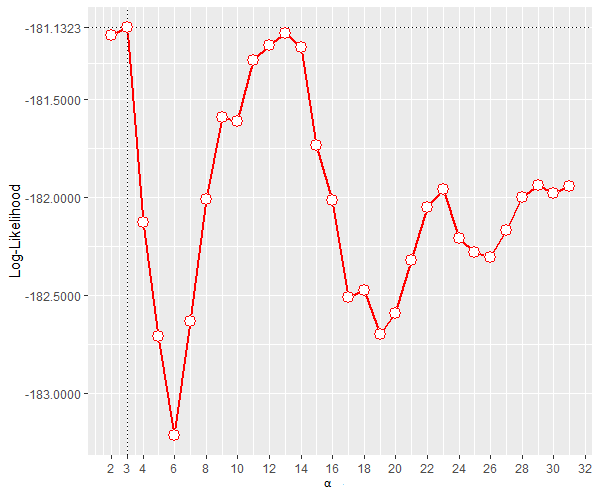
\includegraphics[width=0.49\textwidth]{AlphaBestPlot.png}
    \caption{Plot af likelihoodværdier mod $\alpha$. Parametrene i modellen er estimeret ud fra hver $\alpha$-værdi. Vi ser at den største likelihood opnås ved $\alpha=3$. }
    \label{fig:AlphaPlot}
\end{center}
\end{figure}
\textcolor{blue}{Der er marginal forskel når $\alpha$ går fra 18 til 33}. Denne test gør, at vi i den dynamiske model vælger, at sætte $\alpha=3$ og dermed bruge data fra de 3 forudgående runder til tiden $t$. Hvis vi havde testet tuningstørrelsen over flere sæsoner, vil det være forventeligt at resultatet blev anderledes. Denne forventning bygger blandt andet på, at fodboldklubber ofte køber og sælger spillere fra sæson til sæson.
  \begin{table}[ht]
\centering
\begin{adjustbox}{max width=\textwidth}
\begin{tabular}{|l|rrrr|rrrr|}
\hline
\multicolumn{1}{|l|}{} & \multicolumn{4}{l|}{Rao-Kupper} & \multicolumn{4}{l|}{Dynamisk Model} \\
\hline
Parameter & Estimat & SE &2.5\% &97.5\% & Estimat & SE &2.5\% &97.5\%\\
  \hline
    $\hat{\text{HjemmebaneFordel}}$ & -      & -     &      &            & 0.156 & 0.072  &0.014 & 0.298  \\
    $\hat{\text{SejrStreak}}$       & -      & -     &       &           & -0.195 & 0.107 &-0.404 & 0.014 \\
    $\hat{\text{FifaRating}}$       & -0.316 & 0.707 &-1.702 &1.069      & 0.453 & 0.229  &0.004 & 0.902 \\
    $\hat{\text{Hjørne}}$           & -0.437 & 0.980 &-2.359 &1.484      & 0.305 & 0.293  &-0.269 &0.879\\
    $\hat{\text{Offside}}$          &  0.126 & 0.312 &-0.485 &0.738      & -0.079 & 0.142 &-0.358 &0.200 \\
    $\hat{\text{MålScoret}}$        &  0.259 & 0.480 &-0.682 &1.200      & 0.259 & 0.222  &-0.177 &0.695    \\
    $\hat{\text{MålLukketInd}}$     & -0.683 & 0.541 &-1.744 &0.378      & 0.106 & 0.164  &-0.215 & 0.428\\
    $\hat{\text{Tilskuere}}$        &  0.453 & 0.731 &-0.949&1.885       & -0.147 & 0.207 &-0.552 & 0.259\\
    $\hat{\text{Boldbesiddelse}}$   &  0.210 & 0.488 &-0.746 &1.166      & -0.156 & 0.154 &-0.458 & 0.146\\
    $\hat{\text{Skud}}$             &  0.160 & 0.540 &-0.899 &1.218      & -0.011 & 0.259 &-0.519 & 0.497\\
    $\hat{\text{SkudIndenfor}}$     & -0.395 & 0.770 &-1.904 &1.115      & -0.007 & 0.233 &-0.463 & 0.449\\
    $\hat{\text{Frispark}}$         & -0.214 & 0.418 &-1.033 &0.604      & -0.052 & 0.166 &-0.274 & 0.378\\
    $\hat{\theta}$                  & 1.667  & 0.121 &1.429  &1.904      & 1.657 & 0.122  & 1.419 & 1.896\\
   \hline
\end{tabular}
\end{adjustbox}
\caption{\label{tab:Parameterestimater}\textit{$\hat{\theta}$- og $\hat{\beta}$-koefficienter for sæson 2015 i superligaen, med Rao-Kupper til venstre, og den dynamiske model til højre}}
\end{table}
\\Vi ser i (Tabel \ref{tab:Parameterestimater}), at alle $\beta$'erne i Rao-Kupper har store standardfejl og ikke er signifikante med et signifikansniveau på 5\%. $\hat{\theta}$ er signifikant, hvilket den er pr. definition, eftersom vi har uafgjorte kampe. I den dynamiske model, ser det en smule bedre ud, her er $\hat{HjemmebaneFordel}$, $\hat{FifaRating}$ og $\hat{\theta}$ signifikante med et signifikansniveau på 5\%. For at sikre os at $\hat{\beta}$ estimaterne i de to modeller samlet set er signifikante, udfører vi en kvotienttest for modellernes $\hat{\beta}$-parametre, hvor  \\
$H_0$: $\beta_1=\beta_2=...=\beta_{12} = 0$,\\
teststørrelserne bliver dermed for hhv. den statiske og dynamiske model:\\
\begin{align*}
    -2\text{log}(Q_{sta})&=-2\Big{(}\ell_{sta} (\beta_{H_0}, \hat{\hat{\theta}})-\ell_{sta} (\hat{\beta},\hat{\theta})\Big{)}=-2(-211.233+190.644)=41.177\\
    -2\text{log}(Q_{dyn})&=-2\Big{(}\ell_{dyn} (\beta_{H_0},\hat{\hat{\theta}})-\ell_{dyn} (\hat{\beta},\hat{\theta})\Big{)}=-2(-198.0325+181.0782)=33.909
\end{align*}
Her er vores teststørrelse for $H_0$, ved store stikprøver, approksimativt $\chi^2_{10}$ fordelt for Rao-Kupper og $\chi^2_{12}$ fordelt for den dynamiske. De tilhørende $p$-værdier for den staiske- og dynamiske model er hhv. $0.0006$ og $0.0007$, hvorfor vi afviser nulhypotesen om, at $\beta$'erne er uden betydning for modellen. Vi konkluderer dermed, at der ikke er noget belæg for at fjerne $\beta$-parametrene helt fra modellen. 
\\\\I Tabel \ref{tab:Styrkeestimater} sammenligner vi de to modellers rangering af holdene, og derudfra ser vi, at der er betydelig forskel på de to måder at anvende modellen på. Styrkerne for holdene er udregnet relativt til Hobro. Som forventet, kommer Rao-Kupper tættere på den faktiske rangering af holdene end den dynamiske model gør. Styrken for et hold i den dynamiske model er, er beregnet som et gennemsnit af holdets styrke for alle runderne. De estimerede point, er udregnet ud fra de estimerede sandsynligheder tilhørende hver af kampene, hvor pointene tildeles ved: $3 \cdot p_{i \cdot ij}$ point til hold \textit{i}, $3\cdot p_{j \cdot ij}$ point til hold \textit{j} og $1\cdot p_{0 \cdot ij}$ point til begge hold. Bemærk at summen af de estimerede point ikke er lig summen af de observerede point, dette skyldes, at der er en forskel i antallet af estimerede uafgjorte kampe ift. de observerede uafgjorte kampe. \textcolor{blue}{Den sande sum af point er 552, hvor Rao-Kupper estimere 551.947 og den dynamiske estimere 549.426}.\\
\begin{table}[htb!]
\centering
\begin{adjustbox}{max width=\textwidth}
\begin{tabular}{|hh|hhhh|hhhh|}
\hline
\multicolumn{2}{|h|}{} & \multicolumn{4}{h|}{Rao-Kupper} & \multicolumn{4}{h|}{Dynamisk Model} \\
\hline
Hold & Point & Styrke & SE & Estimeret Point & Rangering & Styrke & SE & Estimeret Point & Rangering \\
  \hline
    FCK & 71 & 11.223 & 5.722 & 71.165 & 1  & 5.945 & 2.694 & 67.082 & 1 \\
    SJE & 62 & 7.048  & 3.463 & 61.029 & 2  & 2.617 & 1.085 & 49.250 & 5 \\
    FCM & 59 & 6.233  & 2.816 & 58.191 & 3  & 3.723 & 1.625 & 58.619 & 2 \\
    BIF & 54 & 5.075  & 2.432 & 53.367 & 4  & 2.987 & 0.880 & 52.143 & 3 \\
    AAB & 50 & 4.674  & 2.284 & 51.418 & 5  & 2.947 & 1.396 & 51.259 & 4 \\
    RFC & 47 & 4.032  & 1.901 & 47.923 & 6  & 2.522 & 0.870 & 49.119 & 6 \\
    OB  & 46 & 3.163  & 1.287 & 42.229 & 8  & 1.654 & 0.619 & 37.709 & 9 \\
    VFF & 40 & 2.880  & 1.335 & 40.068 & 9  & 1.484 & 0.608 & 35.285 & 10 \\
    FCN & 38 & 2.423  & 1.154 & 36.171 & 10 & 1.142 & 0.460 & 30.987 & 11 \\
    AGF & 37 & 3.173  & 1.500 & 42.299 & 7  & 2.057 & 0.739 & 42.903 & 8 \\
    EFB & 30 & 1.744  & 0.071 & 29.161 & 11 & 2.410 & 0.880 & 47.775 & 7 \\
    HOB & 18 & 1.000  & 0.000 & 18.926 & 12 & 1.000 & 0.000 & 27.293 & 12 \\
   \hline   
\end{tabular} 
\end{adjustbox}
\caption{\label{tab:Styrkeestimater}Rangering af holdene i forhold til deres styrker udregnet relativt til Hobro, samt deres forventede antal point ved slutningen af sæsonen}
\end{table}
Det viser sig, at der er markant flere hjemmebanesejre end udebanesejre. Figur \ref{fig:boxplot} viser boxplot af estimerede sandssynligheder mod observerede udfald. Vi ser, at den dynamiske model \ref{fig:boxplotD} estimerer fordelingen af hjemmebanesejre, udebanesejr og uafgjort bedre, i forhold til de faktiske udfald af kampene, end Rao-Kupper \ref{fig:boxplotS}. De stiblede linjer (rød, blå, grøn) viser de observerede middelværdier for hhv (hjemmesejr, udesejr, uafgjort):
\begin{table}[htb!]
\centering
\begin{adjustbox}{max width=\textwidth}
\begin{tabular}{|l|ccc|}
\hline 
 & Hjemmmesejr & Udesejr & Uafgjort \\
 \hline
Observeret & 0.460 & 0.328 & 0.212\\
Rao Kupper & 0.396 & 0.391 & 0.213\\
Dynamisk Rao Kupper & 0.463 & 0.322 & 0.215\\
   \hline   
\end{tabular} 
\end{adjustbox}
\caption{\label{tab:Styrkeestimater}\textit{Procentvise observerede og estimerede udfald for Rao Kupper modellen samt den Dynamiske Rao Kupper Model}}
\end{table}\\
At den dynamiske estimerer den observerede fordeling af (hjemmesejr, udesejr, uafgjort) bedre skyldes at den dynamiske model tager højde for hjemmebanefordelen i igennem $\beta_1$. At den statiske models estimater for hjemmesejrer og udesejrer ikke er ens skyldes at alle hold i sæsonen ikke spiller lige mange hjemme og udebanekampe. Det medfører at modellen vil estimere flere hjemmesejrer, hvis det er de hold med de største styrker, som spiller en ekstra hjemmebane kamp. 
\begin{figure}[h!]
  \centering
  \begin{subfigure}[b]{0.8\linewidth}
    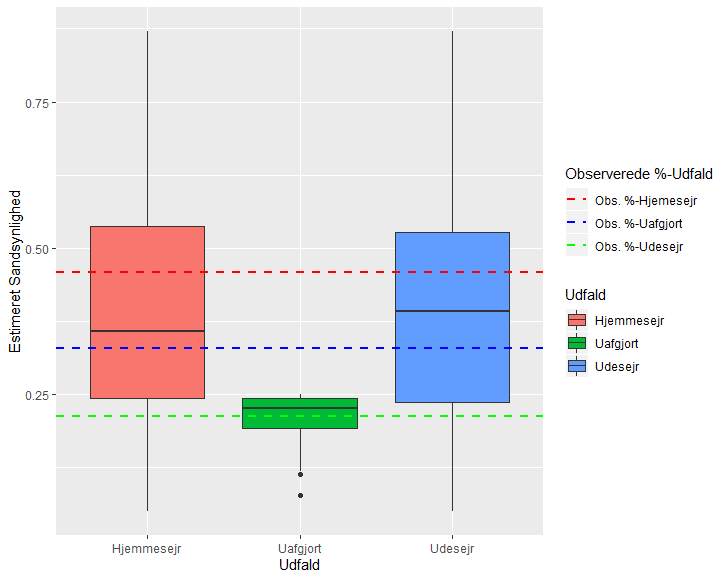
\includegraphics[width=\linewidth]{EstSSHStatisk.png}
    \caption{Statisk}
    \label{fig:boxplotS}
  \end{subfigure}
  \begin{subfigure}[b]{0.8\linewidth}
    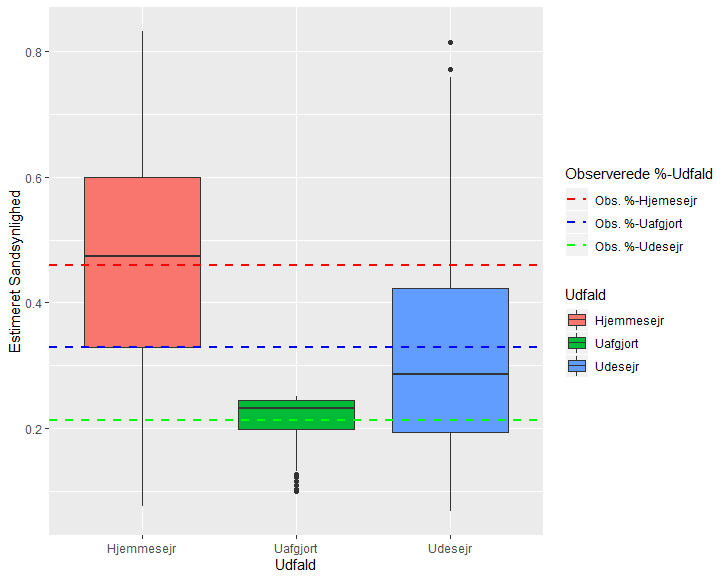
\includegraphics[width=\linewidth]{EstSSHDyn.png}
    \caption{Dynamisk}
    \label{fig:boxplotD}
  \end{subfigure}
  \caption{\textit{Boksplot af estimerede sandsynligheder mod observerede udfald. De røde, blå og grønne boksplot viser fordelingerne af hhv. estimerede hjemmesejrer, udesejrer og uafgjorte kampe. De stiplede linjer viser de emperiske middelværdier for de observerede udfald.}}
  \label{fig:boxplot}
\end{figure}
 \\
 For at se nærmere på de estimerede sandsynligheder, kigger vi på deres respons-residualer mod de fittede værdier for de tre udfald; dette ses i Figur \ref{fig:residualplot}. Den sorte linje viser gennemsnittet af residualerne, og den røde linje er en kerneudglatning med båndbredden 0.06 for hjemme- og udesejr og 0.02 for uafgjort. Båndbredderne er valgt ved at tage udgangspunkt i \textit{R}-funktionen {\fontfamily{qcr}\selectfont dpill}, og efterfølgende rettet til. Vi ser, at middelværdierne for den dynamiske model er tættere på 0 end de er for Rao-Kupper. Rao-Kupper har en middelværdi over 0 for hjemmesejrs residualer og under 0 for udesejrs residualer. Dette er en forventelig følge, da den statiske model generelt vil overestimere sandsynligheden for udesejr og underestimere sandsynligheden for hjemmesejr. Der ser ikke ud til at danne sig noget klart mønster for de fittede værdier, dog er der noget støj ved halerne. Især ved de lave fittede værdier for hjemmesejr, ser vi, at begge modeller har en tendens til at underestimere sandsynligheden, dette er dog meget vægtet af den ene observation i halen. Denne observation kommer fra en kamp mellem Hobro (HOB) og FCK i runde 30, hvor HOB vandt (Hobros dagsform var større end FCKs, på trods af at FCKs forventede styrke var markant større end HOBs). Hvis denne observation blev fjernet, ville kerneudglatningen i den venstre hale være mere flad. Det samme er tilfældet for residualerne tilhørende udesejr for den statiske model, hvor der er en observation der stikker markant ud ved de høje fittede værdier. Det ser lidt kritisk ud for residualerne til hjemmesejr for den dynamiske model, hvor vi får en stigning ved lave fittede værdier. Dette er dog igen kun baseret på 3-4 observationer (hvor FCK mod HOB også indgår), og er derfor svært, at konkludere noget konkret ud fra. Residualerne tilhørende de uafgjorte kampe er meget ens for de to modeller, hvilket også måtte forventes, da $\theta$ er meget ens for dem. Der er dog en lidt større spredning \textcolor{red}{for uafgjort} i de fittede værdier for den dynamiske model, hvilket skyldes \textcolor{red}{forskellen i $\beta$'erne, og især implementeringen af hjemmebanefordelen}. Det er generelt svært at sige noget konkret om disse residualer, eftersom vi har så få observationer i hver kategori. Derfor vælger vi heller ikke at fjerne nogle af de outliers der er beskrevet.
\begin{figure}[h!]
  \centering
  \begin{subfigure}[b]{0.425\linewidth}
    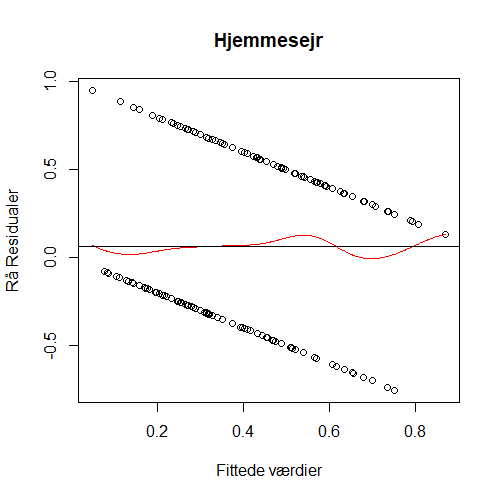
\includegraphics[width=\linewidth]{ResSHS.png}
    \caption{Statisk med båndbredde 0.08}
    \label{fig:ResSHS}
  \end{subfigure}
  \begin{subfigure}[b]{0.425\linewidth}
    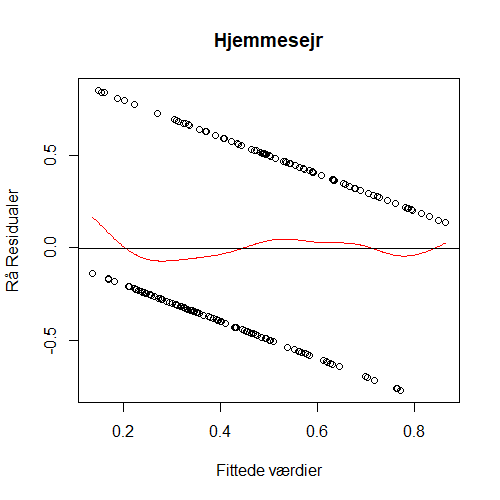
\includegraphics[width=\linewidth]{ResDHS.png}
    \caption{Dynamisk med båndbredde 0.05}
    \label{fig:ResDHS}
  \end{subfigure}
  \begin{subfigure}[b]{0.425\linewidth}
    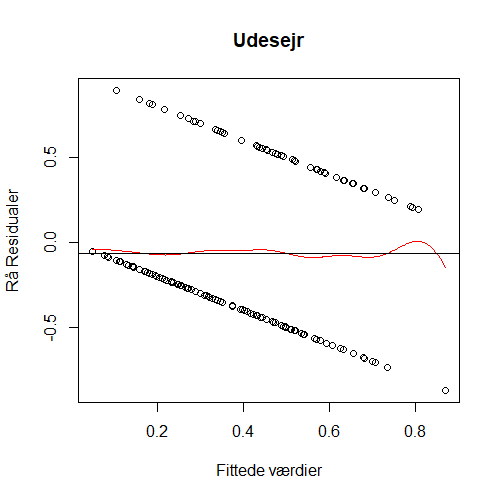
\includegraphics[width=\linewidth]{ResSUS.png}
    \caption{Statisk med båndbredde 0.075}
    \label{fig:ResSUS}
  \end{subfigure}
  \begin{subfigure}[b]{0.425\linewidth}
    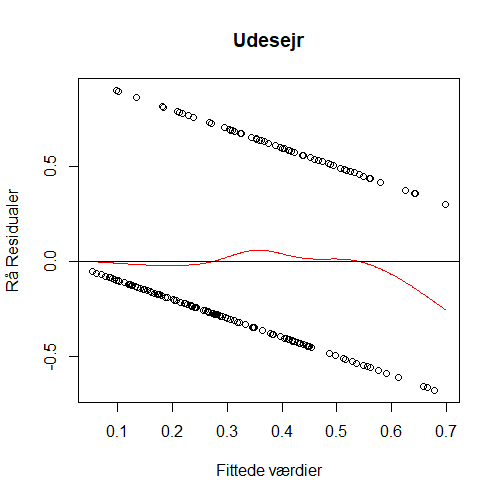
\includegraphics[width=\linewidth]{ResDUS.png}
    \caption{Dynamisk med båndbredde 0.075}
    \label{fig:ResDUS}
  \end{subfigure}
  \begin{subfigure}[b]{0.425\linewidth}
    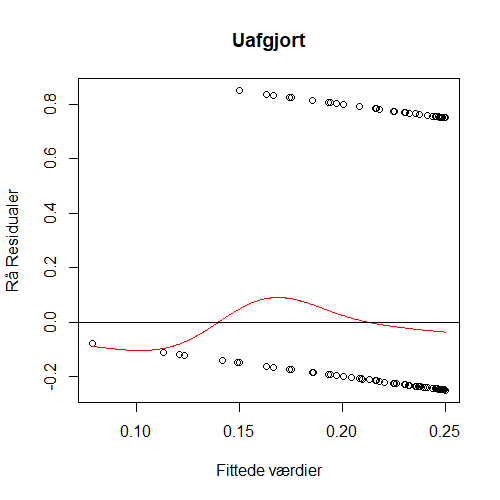
\includegraphics[width=\linewidth]{ResSU.png}
    \caption{Statisk med båndbredde 0.02}
    \label{fig:ResSU}
  \end{subfigure}
  \begin{subfigure}[b]{0.425\linewidth}
    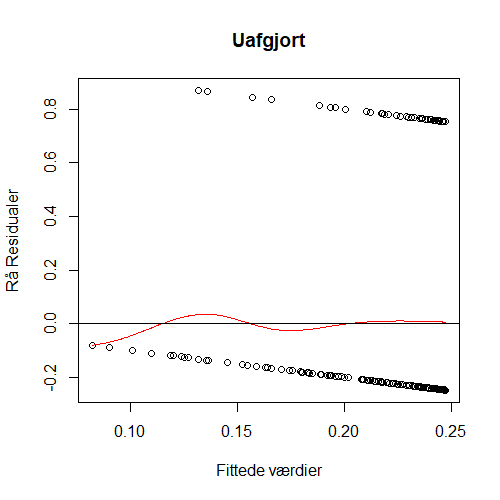
\includegraphics[width=\linewidth]{ResDU.png}
    \caption{Dynamisk med båndbredde 0.02}
    \label{fig:ResDU}
  \end{subfigure}
  \caption{\textit{Residualer mod fittede værdier. Den røde linje viser en Nadaraya-Watson udglatning med normal kerne. De tilhørende båndbredder er valgt med udgangspunkt i R-funktionen dpill, og efterfølgende tilpasset.}}
  \label{fig:residualplot}
\end{figure}
\clearpage
\section{Udvælgelse af parametre}
I dette afsnit viser vi, hvordan vi ved brug lassostraf ($l_1$ norm straf) udvælger de mest beskrivende parametre og sætter deres koefficienter derefter. Formålet er, at forbedre vores models prædiktionsevne ved at mindske modellens forventede prædiktionsfejl eller med andre ord maksimalisere likelihooden på noget fremmed data\\\\
\subsection{Tabsfunktioner}
Når vi beregner prædiktionsfejl, kræver det, at vi noget har testdata som vi ikke har fitted vores model ud fra. Det vil sige, at vi fitter vores model på et træningsdatasæt, for derefter at teste den på et andet testdatasæt. Givet et datasæt med observationerne $\{1,...,N\}$, kalder vi træningsdatasættet for $n$ og testdatasættet for $q$; så $\{1,...,N\}\rightarrow\{1_n,...,N_n,1_q,...,N_q\}$ er en indeksering af observationerne\textcolor{blue}{i forhold til hvorvidt de bliver anvendt til at fitte vores model eller teste den}. En måde, at måle modellens prædiktionsfejl på er \textit{mean squarred prediction error} (MSPE). I MSPE udregnes den kvadrede prædiktionsfejl for hver af sandsynlighederne ($p_{i\cdot ij}, p_{j\cdot ij}, p_{0\cdot ij}$) individuelt, og MSPE for en kamp mellem hold $i$ og hold $j$ bliver så summen af de kvadrede prædiktionsfejlene for hver af de tre estimerede sandsynligheder. MSPE for at hold $i$ vinder over hold $j$ bliver:
\begin{align*}
\text{MSPE}\big{(}\hat{p}_{i\cdot ij}\big{)}=&E\Big{[}\big{(}y_{i\cdot ij}-\hat{p}_{i\cdot ij}\big{)}^2\Big{]}\\
=&E\Big{[}\big{(}\hat{p}_{i\cdot ij}-E\big{[}\hat{p}_{i\cdot ij}\big{]}+E\big{[}\hat{p}_{i\cdot ij}\big{]}-y_{i\cdot ij}\big{)}^2\Big{]}\\
=&E\Big{[}\big{(}\hat{p}_{i\cdot ij}-E\big{[}\hat{p}_{i\cdot ij}\big{]}\big{)}^2+2\big{(}\hat{p}_{i\cdot ij}-E\big{[}\hat{p}_{i\cdot ij}\big{]}\big{)}\big{(}E\big{[}\hat{p}_{i\cdot ij}\big{]}-y_{i\cdot ij}\big{)}\\
&+\big{(} E\big{[}\hat{p}_{i\cdot ij}\big{]}-y_{i\cdot ij}\big{)}^2\Big{]}\\
=&E\Big{[}\big{(}\hat{p}_{i\cdot ij}-E\big{[}\hat{p}_{i\cdot ij}\big{]}\big{)}^2\Big{]}
+2\underbrace{\big{(}E\big{[}\hat{p}_{i\cdot ij}\big{]}-E\big{[}\hat{p}_{i\cdot ij}\big{]}\big{)}}_{0}\big{(}E\big{[}\hat{p}_{i\cdot ij}\big{]}-y_{i\cdot ij}\big{)}\\
&+\big{(} E\big{[}\hat{p}_{i\cdot ij}\big{]}-y_{i\cdot ij}\big{)}^2\\
=&E\Big{[}\big{(}\hat{p}_{i\cdot ij}-E\big{[}\hat{p}_{i\cdot ij}\big{]}\big{)}^2\Big{]}+\Big{(} E\big{[}\hat{p}_{i\cdot ij}\big{]}-y_{i\cdot ij}\Big{)}^2\\
=&Var\Big{(}\hat{p}_{i\cdot ij}\Big{)}+\text{Bias}^2\Big{(}\hat{p}_{i\cdot ij}\Big{)},\\
\intertext{Vi ser at prædiktionsfejlen er en funktion af den kvadrerede bias af vores estimat og variansen af vores estimat. Det vil sige, at vi minimalisere vores prædiktionsfejl ved at minimalisere bias og varians. MSPE for alle de estimerede udfald af kampene mellem hold $i$ og hold $j$ bliver:}
\text{MSPE}\big{(}\hat{p}_{ij}\big{)}&=\text{MSPE}\big{(}\hat{p}_{i\cdot ij}\big{)}+\text{MSPE}\big{(}\hat{p}_{j\cdot ij}\big{)}+\text{MSPE}\big{(}\hat{p}_{0\cdot ij}\big{)},\\
\intertext{ MSPE tabsfunktionen med træningsdatasæt $n$ og testdatasæt $q$ er:}
\mathcal{T}_{\text{MSPE}}\big{(}\hat{\beta}_{-q},\hat{\theta}_{-q}|x,y_{ij},n,q\big{)}&=\frac{1}{N_q}\sum_{t\in q}\sum_{i<j}\big{(}y_{i\cdot ij}(t)-\hat{p}_{i\cdot ij}(t)\big{)}^2+\big{(}y_{j\cdot ij}(t)-\hat{p}_{j\cdot ij}(t)\big{)}^2+\big{(}y_{0\cdot ij}(t)-\hat{p}_{0\cdot ij}(t)\big{)}^2\Big{)},
\end{align*}
hvor $-q$ i $\hat{\beta}_{-q}, \hat{\theta}_{-q}$ viser at parametrene er estimeret uden observationer fra testdatasættet $q$, og $N_q$ er antal observationer i testdatasættet\newline\newline
En anden hyppigt anvendt tabsfunktion i klassificeringsproblemer er \textit{logistic loss}\cite{LineSearch} (log loss) også kendt som \textit{cross entropy loss}. I log loss er den forventede prædiktionsfejlen beregnet i forhold til hvor langt væk den estimerede sandsynlighed for det observerede udfald er fra 1; log loss prædiktionsfejlen i en kamp mellem hold $i$ og hold $j$ i runde $t$ bliver:
\begin{align*}
    \mathcal{T}_{\log} \big{(}p_{ij}(t)\big{)}
    &=-\Big{(}y_{i\cdot ij}(t)\log\big{(}\hat{p}_{i\cdot ij}(t)\big{)}+y_{j\cdot ij}(t)\log\big{(}\hat{p}_{j\cdot ij}(t)\big{)}
    +y_{0\cdot ij}(t)\log\big{(}\hat{p}_{0\cdot ij}(t)\big{)}\Big{)},\\
\intertext{og log tabsfunktionen for hele testsættet bliver:}
\mathcal{T}_{\log}\big{(}\hat{\beta}_{-q},\hat{\theta}_{-q}|x,y_{ij},n,q\big{)}
&=-\frac{1}{N_q}\sum_{t\in q}\sum_{i<j}\Big{(}y_{i\cdot ij}(t)\log\big{(}\hat{p}_{i\cdot ij}(t)\big{)}
+y_{j\cdot ij}(t)\log\big{(}\hat{p}_{j\cdot ij}(t)\big{)}
+y_{0\cdot ij}(t)\log\big{(}\hat{p}_{0\cdot ij}(t)\big{)}\Big{)}.\\
\intertext{Ved at sammenligne med likelihood funktionen ser vi, at minimalisere log tabsfunktionen er ækvivalent med at minimalisere den negative log likelihood (maksimalisere log likelihooden) over testsættet:}
-\ell\big{(}\hat{\beta}_{-q},\hat{\theta}_{-q}\big{)}
&=-\log\prod_{t\in q}\prod_{i<j}\hat{p}_{i\cdot ij}(t)^{y_{i\cdot ij}(t)}\hat{p}_{j\cdot ij}(t)^{y_{j\cdot ij}(t)}\hat{p}_{0\cdot ij}(t)^{y_{0\cdot ij}(t)}\\
&=-\sum_{t\in q}\sum_{i<j}\Big{(}y_{i\cdot ij}(t)\log\big{(}\hat{p}_{i\cdot ij}(t)\big{)}+y_{j\cdot ij}(t)\log\big{(}\hat{p}_{j\cdot ij}(t)\big{)}+y_{0\cdot ij}(t)\log\big{(}\hat{p}_{0\cdot ij}(t)\big{)}\Big{)}.
\end{align*}
\subsection{Lasso}
\textit{"FIND NYT CITAT" - \textcolor{red}{William Shakespeare}.}\\
Indtil videre har vi anvendt alle vores forklarende variable, til at beskrive de forskellige fodboldholds styrker. Der er altså en risiko for, at vi overfitter vores model med overflødige variable, som enten beskriver; den samme varians, beskriver den dårligt, eller slet ikke beskriver den. I dette afsnit vil vi tage udgangspunkt i \textcolor{red}{PSYOKO STAT NØRDs} citat, og forsøge at indskærpe modellen, så de "bedste" variable vægtes mest og de dårligere enten vægtes mindre eller fjernes helt. Robert Tibshirani (1996)\cite{RobertTibshirani} foreslår en metode kaldet lasso \textit{(least absolute shrinkage and selection operator)} til at identificere, hvor godt de forskellige parametre beskriver udfaldene og justerer deres koefficienter derefter. Lasso-optimeringsproblemet tager som tidligere udgangspunkt i maksimalisere likelihooden, men nu under en bibetingelse:
\begin{align*}
&\max_{\beta,\,\theta} \Big{\{}\ell(\beta,\theta)\Big{\}} \\
&\text{u.b.b. }\sum_{i=1}^k|\beta_i|\leq s,
\end{align*}
hvor bibetingelsen straffer i forhold til de normerede $\beta$-koefficienterne. $s$, som beskriver den størst mulige sum af $\beta$-koefficienterne, er en brugervalgt strafparameter. 
Vi omskriver lasso-problemet på \textit{Lagrange-form}, da vi senere hen benytter dets praktiske \textcolor{blue}{anvendelighed /implementerbarhed.}:
\begin{align*}
\max_{\beta,\,\theta} \Big{\{}\ell(\beta,\theta)-\lambda\sum_{i=1}^k|\beta_i|\Big{\}}=\min_{\beta,\,\theta} \Big{\{}-\ell(\beta,\theta)+\lambda\sum_{i=1}^k|\beta_i|\Big{\}},
\end{align*}
hvor $\lambda\geq0$ er en strafparameter tilsvarende $s$, og beskriver hvor objektfunktionen skal straffes i forhold de normerede $\beta$-koefficienter. $\lambda$ og $s$ har et inverst forhold, så når $\lambda$ er høj, er $s$ lav. Hvis $s\geq\sum_i^k\|\beta_i|\iff \lambda=0$ vil lasso løsningen være lig maksimum likelihood løsningen, men hvis $s=\frac{1}{\delta}\sum_i^k\|\beta_i|$ vil koefficienterne gennemsnitligt mindskes til $\frac{1}{\delta}$ af hvad de var før. \textcolor{red}{Sammenhængen mellem $\lambda$ og $s$ er bevist i bevist for en konvex lineær model med ortogonal designmatrice i bevis (REF)}
\subsubsection{Parameterestimering med lassostraf}
\textcolor{blue}{For at forklare effekten af lasso på parametrene, vil vi tage udgangspunkt i en lineær model med ortogonal designmatrice, fordi vi i det tilfælde kan skrive resultatet ned eksplicit. Når X er ortogonal er $X^T=X^{-1}$, så mindste kvadraters løsningen bliver:}
\begin{align*}
\hat{\beta}=\big{(}X^TX\big{)}^{-1}X^Ty=X^Ty.
\end{align*}
Lasso-problemet for en lineær model bliver:
\begin{align*}
&\min_\beta \Big{\{}\big{(}y-X\beta\big{)}^T\big{(}y-X\beta\big{)}+\lambda\sum_{i=1}^k|\beta_i|\Big{\}}=\min_\beta \Big{\{}y^Ty+X^TX\beta^T\beta-2y^TX\beta+\lambda\sum_{i=1}^k|\beta_i|\Big{\}},\\
\intertext{thi $y^Ty$ er uafhængig af $\beta$, $X^TX=1$ og $\hat{\beta}=X^Ty$ omskriver vi problemet til:}
&\min_\beta \Big{\{}2\beta^2-\hat{\beta}\beta+\lambda\sum_{i=1}^k|\beta_i|\Big{\}}=\min_\beta \Big{\{}\sum_{i=1}^k\Big{(}2\beta_i^2-\hat{\beta_i}\beta_i+\lambda |\beta_i|\Big{)}\Big{\}}.\\
\intertext{Objektfunktion er nu en sum af k identiske problemer, som vi løser hver for sig. Vi tager udgangspunkt i det i'te problem, og får objektfunktionen:}
&f(\beta_i)=-2\hat{\beta}_i\beta_i+\beta_i^2+\lambda|\beta|.\\
\intertext{Thi vi ønsker at minimere objektfunktionen må det gælde, at $\hat{\beta}_i>0\rightarrow\beta_i\geq0$, for ellers ville objektfunktionen kunne mindskes ved at skifte fortegnet for $\beta_i$, og ligeledes må det gælde, at $\hat{\beta}_i<0\rightarrow\beta_i\leq0$ Ved at differentier og sætte lig 0 fås den afledte:}
&f'(\beta_i)=-2\cdot\text{sign}\big{(}\hat{\beta_i}\big{)}\hat{\beta_i}+2\beta_i+\lambda. \\
\intertext{Ved at isolere $\beta_i$ og gange begge sider med fortegnet for $\beta_i$ (fortegnet for $\hat{\beta_i}$), for at sikre positivt fortegn på venstre siden, fås:}
&\beta_i=\text{sign}\big{(}\hat{\beta_i}\big{)}\Big{(}\text{sign}\big{(}\hat{\beta_i}\big{)}\hat{\beta_i}-\frac{1}{2}\lambda\Big{)}=\text{sign}\big{(}\hat{\beta_i}\big{)}\big{(}|\hat{\beta_i}|-\frac{1}{2}\lambda\big{)},\\
\intertext{hvis $\hat{\beta}_i<0$ kræves, at $\text{sign}\big{(}\hat{\beta_i}\big{)}\big{(}|\hat{\beta_i}|-\frac{1}{2}\lambda\big{)}\leq0$ og ligeledes kræver $\hat{\beta}_i>0$, at $\text{sign}\big{(}\hat{\beta_i}\big{)}\big{(}|\hat{\beta_i}|-\frac{1}{2}\lambda\big{)}\geq0$, hvilket løses ved at sætte $\big{(}|\hat{\beta_i}|-\frac{1}{2}\lambda\big{)}$ lig nul, hvis ledet er negativt:}
&\hat{\beta}_i^{\text{lasso}}=\text{sign}\big{(}\hat{\beta_i}\big{)}\big{(}|\hat{\beta_i}|-\frac{1}{2}\lambda\big{)}^{+},\\
\intertext{så}
&\hat{\beta}^{\text{lasso}}=\sgn\big{(}\hat{\beta}\big{)}\big{(}|\hat{\beta}|-\frac{1}{2}\lambda\big{)}^{+}
\end{align*}
Vi ser tydeligt, at når $\lambda$ stiger, går $\hat{\beta}_i^{\text{lasso}}$ mod 0, samt at $\lambda\geq2|\hat{\beta}_i|\rightarrow \hat{\beta}_i^{\text{lasso}}=0$. Det vil sige, at i forbindelse med at $\lambda$ stiger vil lasso-estimaterne gå mod 0, samt at når $\lambda$ bliver tilpas stor vil en eller flere koefficienter sættes lig 0, hvilket betyder at lasso løbende træffer et valg af underum. Idéen er nu, at når $|\beta|$-koefficienterne mindskes, mindskes variansen af de estimerede sandsynligheder, hvilket medfører at modellens prædiktionsfejl mindskes. Dette sker dog på bekostning af, at når $|\beta|$-koefficienterne mindskes, medfører det også at den kvadrerede bias stiger, hvilket øger modellens forventede fejl. Variansen falder, da sandsynlighederne bliver mindre påvirket af deres kovariater. Den kvadrerede bias stiger, da lasso trækker estimaterne mod 0 og væk fra de centrale løsninger. Ved justering af $\lambda$ bliver modellens forventede prædiktionsfejl altså trukket i hver sin retning på grund af ændringer i bias og varians. Dette forhold mellem bias og varians kaldes \textit{The Bias-Variance Decomposition}\cite{ESL}. Humlen er så, at finde den $\lambda$ der minimerer de forventede prædiktionsfejl.
\subsection{LAMBDA OG S}
Med udgangspunkt i en lineær model som tidligere: Lad $f:\Reals^k\rightarrow R$ være en konveks funktion, så vil for et hvilket som helst par af vektorer $(\beta, \hat{\beta})$ i $f$'s mængde og for en $b\in [0,1]$ gælde, at
\begin{align*}
    f(b\beta+(1-b)\hat{\beta})\leq bf(\beta)+(1-b)f(\hat{\beta}),
\intertext{hvilket betyder, at en linje mellem to $f(\beta)$ og $f(\beta')$ altid vil ligge på eller over grafen for f. Det medfører, at hvis en konveks funktion har et lokalt minimumspunkt er det også et globalt minimumspunkt. $\hat{\beta}$ er globalt minimumspunkt, hvis}
    bf(\beta)+(1-b)f(\hat{\beta})\leq bf(\beta)+(1-b)f(\beta),
\intertext{}
\end{align*}

\textit{least squares} tabsfunktionmed minimumspunkt $\hat{\beta}$. Lad $|\Tilde{\beta}|<s$. for $b\in [0,1]$ 


\subsection{$\lambda$ og s forhold}
I løsningen til lasso problemet gælder bibetingelsen:
\begin{align*}
&\sum_i^k|\hat{\beta}^{\text{lasso}}|
\leq s
\intertext{Det må gælde, at hvis:}
&s\leq\sum_i^k|\hat{\beta}_i|=\|\hat{\beta}\|
\intertext{så er}
&s=\|\hat{\beta}^{\text{lasso}}\|
\intertext{fordi ellers eksistere der en $\hat{\hat{\beta}}^{\text{lasso}}$, som opfylder:} 
&\|\hat{\beta}^{\text{lasso}}\|<\|\hat{\hat{\beta}}^{\text{lasso}}\|\leq s 
\intertext{hvilket betyder, at $\hat{\hat{\beta}}^{\text{lasso}}$ er tættere på den centrale løsning $\hat{\beta}$ end $\hat{\beta}^{\text{lasso}}$, så:}
&\ell\big{(}\hat{\theta},\hat{\hat{\beta}}^{\text{lasso}}\big{)}>\ell\big{(}\hat{\theta},\hat{\beta}^{\text{lasso}}\big{)}.
\intertext{Det medfører, at når $0 < s  < \|\hat{\beta}\|$ er}
&s=\|\hat{\beta}^{\text{lasso}}\|=\|\big{(}|\hat{\beta}|-\frac{1}{2}\lambda\big{)}^{+}\|,
\intertext{hvorfra vi tydeligt ser, at der er en én til én korrespondance mellem $s$ og $\lambda$, hvor at når $\lambda$ er høj, er s lav, samt $s\geq \hat{\beta}\iff \lambda=0$, hvor $\hat{\beta}^{\text{lasso}}=\hat{\beta}$}
\end{align*}

\subsection{Implementering af lasso}
Ændringerne i de estimerede sandssynligheder ved implementering af lasso sker i det $\hat{\beta}^{\text{lasso}}$-koefficienterne bliver funktioner af $\lambda$. \textcolor{blue}{som vist i afsnit 4.1.1, hvor vi udleder estimaterne.} I den dynamiske Rao-Kupper model med lasso-straf opskriver vi den forventede sandsynlighed for at hold $i$ vinder over hold $j$ som:
\begin{align}
    \hat{p}^{\text{lasso}}_{i\cdot ij}(t)=P\big{\{}\hat{Y}_{i}(t)>\hat{Y}_{j}(t)\big{\}}
    &=\frac{\hat{\pi}_i\big{(}x_i(t,\alpha),\hat{\beta}(\lambda)\big{)}}{\hat{\pi}_i\big{(}x_i(t,\alpha),\hat{\beta}(\lambda)\big{)}+\hat{\theta}\hat{\pi}_j\big{(}x_j(t,\alpha),\hat{\beta}(\lambda)\big{)}}\\
    &=\frac{1}{1+e^{-\big{(}x_i^T(t,\alpha)\hat{\beta}(\lambda)-x_j^T(t,\alpha)\hat{\beta}(\lambda)-\eta\big{)}}}.
    \label{func:pdynlasso}
\end{align}
\textcolor{blue}{Da Newton-Rhapson algoritmen kræver at funktionen der ønskes maksimaliseret er to gange differentiabel og strafledet $\lambda |\beta|$ kun er én gang differentiabel med hensyn til $\beta$, approksimerer vi strafledet med den glatte funktion $\lambda(\sqrt{\beta^2+C^2})\approx\lambda |\beta|$ når $C\rightarrow 0$, for forsat at anvende Newton-Rhapson algoritmen til at estimere vores parametre. Bemærk at vi i resten af projektet refererer til dette strafled som lasso, på trods af at det er en approksimation. Maksimaliseringsproblemet til estimering og udvælgelse af parametre bliver:}
\begin{align*}
\max_{\beta,\,\theta} &\Big{\{}\ell\Big{(}\beta,\theta\Big{|}x(t,\alpha),y_{ij}(t),r_{ij}(t)\Big{)}-\lambda \Big{(}\sqrt{\beta^2+C^2}\Big{)}\Big{\}}\\
=\max_{\beta,\,\theta} 
&\Big{\{}\sum_{t}\sum_{i<j}\Big{[}y_{i\cdot ij}(t)\log\Big{(}\frac{\pi_i}{\pi_i+\theta\pi_j}\Big{)}
+ y_{j\cdot ij}(t)\log\Big{(}\frac{\pi_j}{\pi_j+\theta\pi_i}\Big{)}\\
&+ \big{(}r_{ij}(t)-y_{i\cdot ij}(t)-y_{j\cdot ij}(t)\big{)} \log\Big{(}\frac{(\theta^2-1)\pi_i \pi_j}{(\pi_i+\theta\pi_j)(\pi_j+\theta\pi_i)}\Big{)}\Big{]}-\lambda \Big{(}\sqrt{\beta^2+C^2}\Big{)}\Big{\}},
\end{align*}
\textcolor{blue}{hvor $\pi_i=\pi_i\big{(}x_i^T(t,\alpha),\beta(\lambda)\big{)}$. For at gøre konvergeringen hurtigere initialiseres problemet med $\beta=\hat{\beta}_0$ og $\theta=\hat{\theta}_0$. Udvælgelsen af parametrene sker ved baglæns elimination, hvor vi initialisere med samtlige parametre og efterfølgende fjerner dem hvis de bliver 0. Idet vi løser problemet numerisk er det nødvendigt, at have en grænseværdi for, hvornår vi anser en parameter tæt nok på 0 til at være 0. Efter\textit{trial and error}, synes vi, at en nedre grænseværdi på $10^{-5}$ for parametrene resultere i en fornuftig spredning af fravælgelsen; så hvis $\beta_k<10^{-5}$ eller fortegnet for $\beta_k$ ændres ved en konvergering, sættes $\beta_k=0$. Hvis grænsen sættes meget strengere vil parametrene kunne sættes markant under vores Newton-Rhapson konvergerings tolorence for samlet ændring i parametrene på $10^{-6}$, og derfor ikke blive fjernet. Hvis grænsen sættes meget mildere vil de fleste parametre være fjernet allerede ved meget lave $\lambda$ værdier og det vil derfor være svært at skelne mellem hvor godt de forskellige parametre beskriver styrkerne. Figur \ref{fig:DBetaLasso} viser $\hat{\beta}^{\text{lasso}}$-koefficienterne mod $\lambda$ i den dynamiske model og den tilhørende algoritme til estimering og udvælgelse parametrene er skrevet som pseudokode i \textit{Algorithm 3}}\\
\sout{Til at implementere lasso-straffen, approksimerer vi strafledet med en glat udgave, \textcolor{blue}{hvorved vi sørger for at den er differentiabel}, $\lambda |\beta| = \lambda(\sqrt{\beta^2+C^2})$ hvor vi lader $C\rightarrow 0$. Vi kan dermed ikke antage at vores estimerede \textcolor{blue}{parameterkoefficienter} bliver lig 0, og derfor sætter vi en grænse for hvor tæt de må være på 0, før vi fjerner dem. Denne grænse skal selvfølgelig være så lav at det giver mening at fjerne dem, hvorfor vi vælger at sætte $\beta_k$ lig 0 og dermed fjerne den når $\beta_k<10^{-6}$. Derudover sætter vi også $\beta_k = 0$, i situationen hvor $\beta_k<10^{-5}$ samt at den skifter fortegn i den efterfølgende iteration. Dette gøres, under tesen om at parameteren er uden betydning, eftersom den gennemsnitligt ligger meget tæt på 0\textcolor{blue}{vagt argument}. Eftersom vi fjerner en parameter når den skifter fortegn, er det vigtigt at de initialiseringsværdier vi vælger har de fortegn, som vi forventer de konvergerer mod. Derfor vælger vi at initialisere $\beta_0$ og $\theta_0$, med $\hat{\beta}_{MLE}$ og $\hat{\theta}_{MLE}$ estimaterne for $\lambda=0$. Hvilket vil sige at vi estimerer $\beta$'erne ud fra baglænselimination, hvor vi altså starter med samtlige $\beta$'er for hver $\lambda$ vi tester.
Algoritmen til at estimere parametrene med lasso-straf, kan læses som pseudokode i \textit{Algorithm 3}}.\\
\begin{algorithm}[H]
\SetAlgoLined
\KwResult{$\max_{\beta,\,\theta} \Big{\{}\ell\Big{(}\beta,\theta|x,y_{ij}(t),r_{ij}(t),\lambda\Big{)}\Big{\}}$}
 Initialisér $v_0 = \begin{bmatrix}
           \beta \\
           \theta
         \end{bmatrix} =\begin{bmatrix}
           \beta_0 \\
           \theta_0
         \end{bmatrix}\;$\\
 \For{($c = 0,1,..., $ indtil konvergens)}{
  \For{$(t = 3,...,SlutRunde)$}{
        \eIf{($\alpha\geq t$)}{$\alpha_1 = t-1\;$}{$\alpha_1 = \alpha\;$}
        $L(\beta_c,\theta_c) = L(\beta_c,\theta_c) + \sum_{c = t-\alpha_1}^{t-1}\sum_{i<j}\ell\Big{(}\beta,\theta,\Big{|}x(t,\alpha),y_{ij}(t),r_{ij}(t),\lambda\Big{)}$\;
    }
        $s_c = s_c + \nabla L\Big{(}\beta_c,\theta_c\Big{)}$\;
        $i_c = i_c + \Big{(}-\nabla^2 L(\beta_c,\theta_c)\Big{)}$\;
\eIf{($i_c$ er positiv semi definit)}{
    \For{(N = 1,...,100)}{
    $\omega = \frac{1}{\text{\mathcal{N}}}$\;
    $\begin{bmatrix}
       \beta_{c+1} \\
       \theta_{c+1}
    \end{bmatrix} = v_{c+1} = v_c + i_c^{-1}s_c\omega$\;
        \If{$(L(\beta_{c+1},\theta_{c+1})>L(\beta_c,\theta_c))$}
        {\textbf{break}\;}
    }
    }{
    \textbf{return}($v_c$)\;
   }
\For{($k = 1,...,length(\beta)$)}{
    \If{($(abs(\beta[k]_{c+1}) < 10^{-6})$ \|\; $(\text{sign}(\beta[k]_{c})\neq \text{sign}(\beta[k]_{c+1})$ \& $\text{abs}(\beta[k]_{c+1})<10^{-5})$)}{$\beta[k] = 0$\;}
    }
 }
\caption{Newton-Raphson for Dynamisk Model med lasso-straf}
\label{alg: DYNLASSO}
\end{algorithm}
\section{Modelovervejelser og model udvælgelse}
I dette afsnit gennemgår vi krydsvalidering, som bruges til at opdele vores datasæt, så vi kan bruge det til at bestemme den optimale $\lambda$-værdi. Dermed opdeler vi vores datasæt i en test og en træningsdel, og bestemmer vores $\lambda$-værdi ud fra MSPE og Log-Loss prædiktionsfejlene. Efter vi har bestemt $\lambda$-værdien, fitter vi vores modeller på det fulde datasæt og tester dem på data fra Superligaen sæson 2014-2015. 

\subsection{Krydsvalidering}
For at udvælge størrelsen af vores strafparameter $\lambda$ benytter vi os af krydsvalidering, som bruges til sammenligne prædiktionsfejlene for modellen for forskellige $\lambda$ værdier. Først deler vi datamængden op i $Q$ lige store dele, hvor vi lader $q\in \{q_1,...,q_Q\}$ betegne de forskellige delmægnder; dermed bliver $\{1,...,N\}\rightarrow\{q_1,...,q_Q\}$ en indeksering af det fulde datasæt. Vi kalder nu træningsdatasættet for $n_q$, som beskriver det fulde datasæt fratrukket den $q$'te mængde, og testdatasættet bliver så den $q$'te mængde, som ikke er inkluderet i træningsdatasættet. Idéen ved krydsvalidering er nu, at vi kan teste hele datamængden, ved at ændre hvilken delmængde der ønskes testet og dermed også ændre hvilke mængder modellen bliver fitted til. Vi benttter dermed hver delmængde som testdatasæt én gang. Den estimerede prædiktionsfejl ved krydsvalidering for vores model bliver dermed et gennemsnit
af prædiktionsfejlene for hver testet spillerunde. 
\begin{align*}
KV\big{(}\ell_{\text{dyn}}(\hat{\beta},\hat{\theta})\big{)}&=\frac{1}{N}\sum_{q=q_1}^{q_Q}\mathcal{T}\big{(}\hat{\beta}_{-q},\hat{\theta}_{-q}|x,y_{ij}\big{)},\\
\intertext{og for et givet strafparameter $\lambda_i$:}
KV\big{(}\ell_{\text{dyn}}(\hat{\beta},\hat{\theta}),\lambda_i\big{)}&=\frac{1}{N}\sum_{q=q_1}^{q_Q}\mathcal{T}\big{(}\hat{\beta}_{-q},\hat{\theta}_{-q}|x,y_{ij},\lambda_i\big{)}
\end{align*}
Da vi ønsker at minimalisere krydsvaliderings prædiktionsfejlen, vælges $\lambda$ ud fra minimaliseringsproblemet:
\begin{align*}
&\min_{\lambda}\Big{\{}KV\big{(}\ell_{\text{dyn}}(\hat{\beta},\hat{\theta}),\lambda \big{)}\Big{\}}=\min_{\lambda}\Big{\{}\frac{1}{N}\sum_{q=q_1}^{q_Q}\mathcal{T}\big{(}\hat{\beta}_{-q},\hat{\theta}_{-q}|x,y_{ij},\lambda\big{)}\Big{\}},\\
\intertext{som ved brug af MSPE-tabsfunktion:}
&\min_{\lambda}\Big{\{}\frac{1}{N}\sum_{q=q_1}^{q_Q}\sum_{t\in q}\sum_{i<j}\Big{[}\big{(}y_{i\cdot ij}(t)-\hat{p}_{i\cdot ij}(t)\big{)}^2+\big{(}y_{j\cdot ij}(t)-\hat{p}_{j\cdot ij}(t)\big{)}^2+\big{(}y_{0\cdot ij}(t)-\hat{p}_{0\cdot ij}(t)\big{)}^2\Big{]}\Big{\}}\\
\intertext{eller ved brug af log-tabsfunktion:}
&\min_{\lambda}\Big{\{}\frac{1}{N}\sum_{q=q_1}^{q_Q}\sum_{t\in q}\sum_{i<j}-\Big{[}y_{i\cdot ij}(t)\log\big{(}\hat{p}_{i\cdot ij}(t)\big{)}+y_{j\cdot ij}(t)\log\big{(}\hat{p}_{j\cdot ij}(t)\big{)}+y_{0\cdot ij}(t)\log\big{(}\hat{p}_{0\cdot ij}(t)\big{)}\Big{]}\Big{\}},
\end{align*}
hvor de estimerede sandsynligheder, beregnet som i (\ref{func:pdynlasso}), er funktioner af $\lambda$.
\subsection{Estimater - find titel}
For at få en idé om hvordan vores parametre ($\beta$) opfører sig for givne $\lambda$'er, har vi i figurene (\ref{fig:DBetaLasso}) og (\ref{fig:StatiskLine}) visualiseret de estimerede $\beta$-koefficienter i forhold til $\lambda$-værdierne for henholdsvis Den Dynamiske Rao Kupper Model og Rao Kupper Modellen  begge uden krydsvalidering. På Figur (\ref{fig:DBetaLasso}) ses det at især kovariaterne Mål, FifaRating og HjemmeBane kræver en høj $\lambda$-værdi før de sættes lig 0. Hvorimod syv af kovariaterne bliver sat lig 0 i intervallet $\lambda \in [0,5]$. Generelt ses det på figuren, at koefficienterne falder stødt når $\lambda$ stiger. Koefficienterne for (den generelle) Rao Kupper Modellen i Figur  \ref{fig:StatiskLine}, er mere delte, i form af at syv af parametrene bliver sat lig nul for $\lambda<1$, hvorefter Mål, MålLukketInd og Tilskuere stort set ikke ændrer sig efterfølgende. At kovariaterne Mål og MålLukketInd ikke bliver sat lig nul, skyldes at der er store korrelation mellem målforskel og slutplacering i ligaen, og eftersom denne model prædikterer ud fra det fulde data vil de to kovariater have stor betydning.
\begin{figure}[h!]
  \centering
  \begin{subfigure}[b]{0.425\linewidth}
    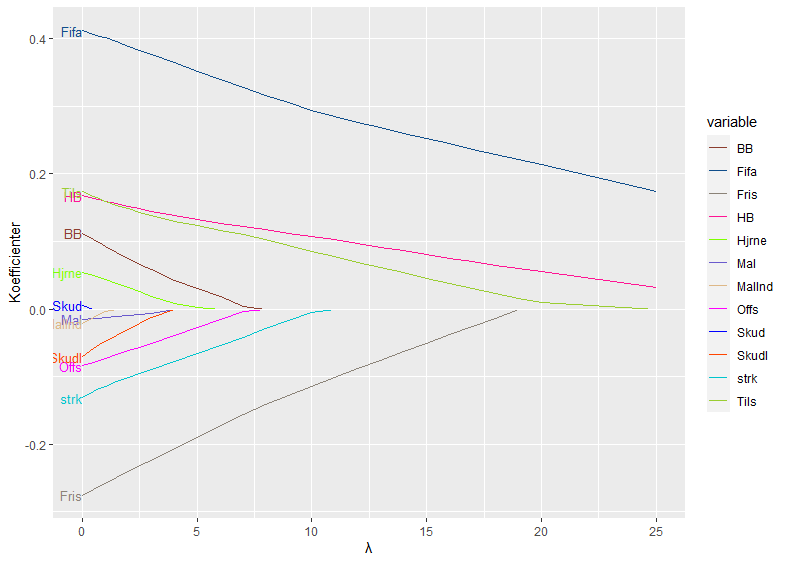
\includegraphics[width=\textwidth]{LINEPLOTDYNALPHA.png}
    \caption{$\hat{\beta}^{\text{lasso}}$-koefficienter for forskellige straf-størrelser i den Dynamiske Rao Kupper Model med lasso-straf}
    \label{fig:DBetaLasso}
  \end{subfigure}
  \begin{subfigure}[b]{0.425\linewidth}
    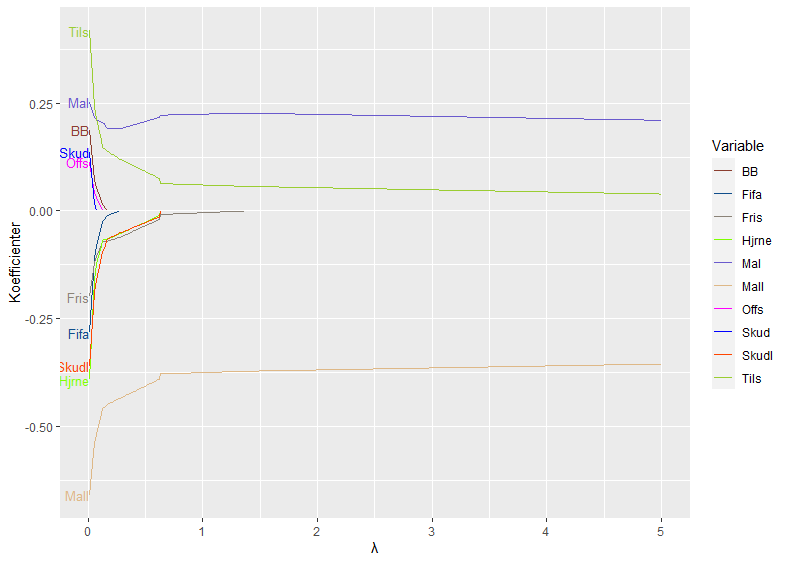
\includegraphics[width=\textwidth]{SKL2.png}
    \caption{$\hat{\beta}^{\text{lasso}}$-koefficienter for forskellige straf-størrelser i Rao Kupper Modellen med lasso-straf}
    \label{fig:StatiskLine}
  \end{subfigure}
\caption{\textit{Estimerede koefficienter mod $\lambda$-værdier for Den Generelle Rao Kupper Model og Den Dynamiske Rao Kupper Model}}
  \label{fig:KoefficienterLambda}
\end{figure}
\\Eftersom målet er at minimere vores prædiktionsfejl, skal vi udvælge den $\lambda$, der minimerer dem, hvilket vi som tidligere beskrevet gør brug af krydsvalidering. Vi har valgt at dele datasættet op i 6 lige store dele, hvor vi prædikterer 5 runder ad gangen. Inddelingerne af runderne er som følgende; $\{4,8\},\{9,13\},\{14,18\},\{19,23\},\{24,28\},\{29,33\}$. Detter er gjort for begge modeller for at kunne sammenligne deres prædiktionsfejl. For hvert interval estimerer vi $\hat{\beta}$ med lasso-straffen $\lambda \in \{0,1,...,30\}$ for den Dynamiske Rao Kupper Model og $\lambda \in \{0,...,6\}$ for den Generelle Rao Kupper Model. For hver opdeling fitter vi modellerne og udregner MSPE og Log-Loss for hver af de udeladte runder. Hver gang vi fjerner en parameter vil denne parameter forblive fjernet, og dermed ikke testet for de resterende $\lambda$'er. Figurene \ref{fig:DynLogLossLine},  \ref{fig:DynMSPELine}, \ref{fig:LogLossStat} og \ref{fig:MSPEStat} viser prædiktionsfejlene, hvor hver linje på graferne repræsenterer prædiktionsfejlene i forhold til $\lambda$ tilhørende én kamp, hver linje er altså bestående af  prædiktionsfejl. \sout{De markante hak i alle graferne, skyldes vores selektering hvor der er fjernet en til flere parametre ved hvert af hakkene.} Vi ser på Figur (\ref{fig:DynMSPELine}) og (\ref{fig:DynLogLossLine}) at variansen i prædiktionsfejlene klart er faldende når $\lambda$ stiger, hvilket også var forventeligt jvf. Bias-Variance tradeoff'et, derudover er det også en naturlig følge da $\hat{\beta} \rightarrow 0 \Rightarrow \pi_i \approx \pi_j \Rightarrow \hat{p}_{i\cdot ij} \approx \hat{p}_{j \cdot ij}$. Det ses på figurene at nogle af linjerne ser ud til ikke at blive påvirket af $\lambda$, og det viser sig også at det er de uafgjorte kampe. På trods af at vores estimerede $\beta$ koefficienter går mod $0$, og vores styrker dermed bliver tættere på hinanden, forbliver de estimerede sandsynligheder for uafgjort ikke ændret markant. Vi ser faktisk at fejlene til de uafgjorte kampe stiger en smule, hvilket må forventes når $\beta$-koefficienterne falder, eftersom $\p_{0 \cdot ij}$ for et fast $\theta$ er maksimeret når $\hat{p}_{i\cdot ij} = \hat{p}_{j \cdot ij}$. Udviklingen af prædiktionsfejlene for Rao Kupper modellen i Figur \ref{fig:MSPEStat} og \ref{fig:LogLossStat} ændrer sig stort set ikke når $\lambda$ stiger, hvilket følger den udvikling vi så i Figur \ref{fig:StatiskLine}. Det tyder altså på at lasso-straffen, ikke har en lige så stor betydning for Rao Kupper modellen, som den har i den Dynamiske model. Dette underbygges yderligere når vi kigger på Figurene \ref{fig:MSPEBarDyn}, \ref{fig:LogLossBarDyn}, \ref{fig:MSPEBarStat} og \ref{fig:LogLossBarStat} hvor vi kan se at de gennemsnitlige prædiktionsfejl i den Dynamiske Model ses at være minimeret for $\lambda = 3$ hvorefter de stiger, og i Rao Kupper modellen stort set ikke ændres, men er minimeret for $\lambda = 0.94$. Det ses yderligere at for $\lambda = 0$ har Rao Kupper modellen lavere prædiktionsfejl end den Dynamiske model, hvorfor lasso-straffen klart forbedrer den Dynamiske model mere end den forbedrer Rao Kupper modellen, dette forhold ses også i Table \ref{tab:KVMSPELOGLOSS}. \\
\begin{figure}[h!]
  \centering
  \begin{subfigure}[b]{0.425\linewidth}
    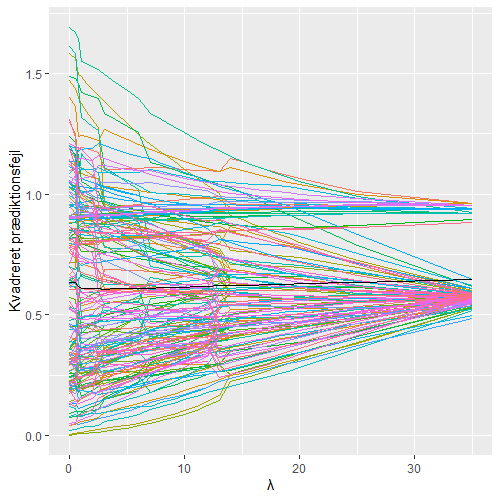
\includegraphics[width=\textwidth]{MSPELINEALPHA.png}
    \caption{Kvadreret prædiktionsfejl mod $\lambda$ for den dynamiske model med lasso-straf, hvor hver linje viser fejlene tilhørende én kamp, og den sorte linje viser gennemsnittet af fejlene, altså MSPE}
    \label{fig:DynMSPELine}
  \end{subfigure}
     \hspace{0.2cm}
  \begin{subfigure}[b]{0.425\linewidth}
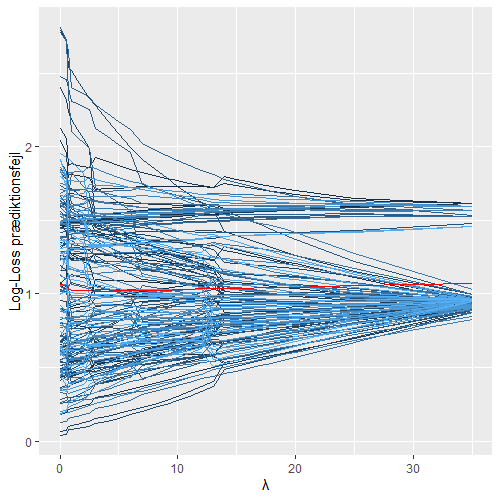
\includegraphics[width=\textwidth]{LINELOGLOSSALPHA.png}
    \caption{Log-prædiktionsfejl mod $\lambda$ for den dynamiske model med lasso-straf, hvor hver linje viser fejlene tilhørende én kamp, og den røde linje viser gennemsnittet af fejlene}
    \label{fig:DynLogLossLine}  
    \end{subfigure}
  \begin{subfigure}[b]{0.425\linewidth}
    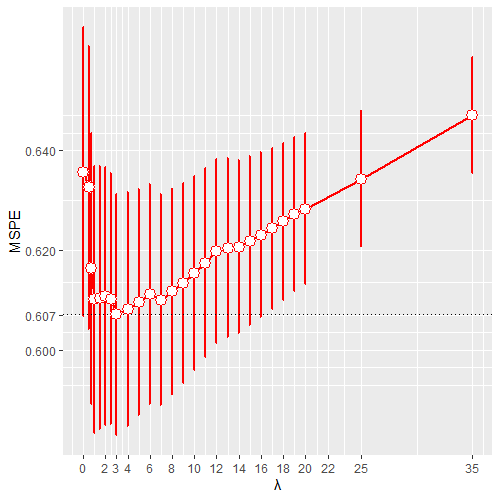
\includegraphics[width=\textwidth]{BARMSPENYALPHA.png}
    \caption{Zoomet ind på den sorte linje i ovenstående figur, viser altså MSPE for hver $\lambda$. Hver ende på barene er en standardfejl fra MSPE'en for den dynamiske model med lasso-straf}
    \label{fig:MSPEBarDyn}
  \end{subfigure}
      \hspace{0.2cm}
    \begin{subfigure}[b]{0.425\linewidth}
    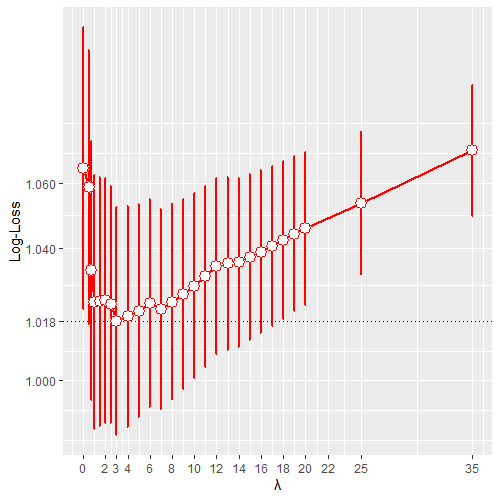
\includegraphics[width=\textwidth]{BARPLOTLOGALPHANY.png}
    \caption{Zoomet ind på den røde linje i ovenstående figur, viser altså gennemsnitlig Log-Loss for hver $\lambda$. Hver ende på barene er en standardfejl fra gennemsnittet for den dynamiske model med lasso-straf}
    \label{fig:LogLossBarDyn}    
    \end{subfigure}
\caption{\textit{MSPE og Log-Loss fra Kryds-Validering i den Dynamiske Rao Kupper Model}}
  \label{fig:MSPELOGLOSDYN}
\end{figure}
%FIGUR TIL STATISK RAO KUPPER
\begin{figure}[htb!]
  \centering
  \begin{subfigure}[b]{0.4\textwidth}
        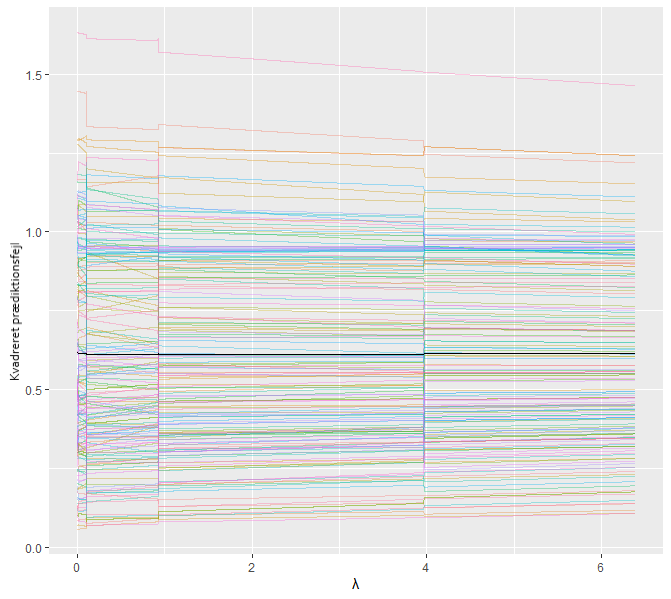
\includegraphics[width=\textwidth]{MSPESTATISK1.png}
    \caption{Kvadreret prædiktionsfejl mod $\lambda$ for den Generelle Rao Kupper Model med lasso-straf, hvor hver linje viser fejlene tilhørende én kamp, og den sorte linje viser gennemsnittet af fejlene, altså MSPE}
    \label{fig:MSPEStat}
  \end{subfigure}
  \hspace{0.2cm}
  \begin{subfigure}[b]{0.4\textwidth}
    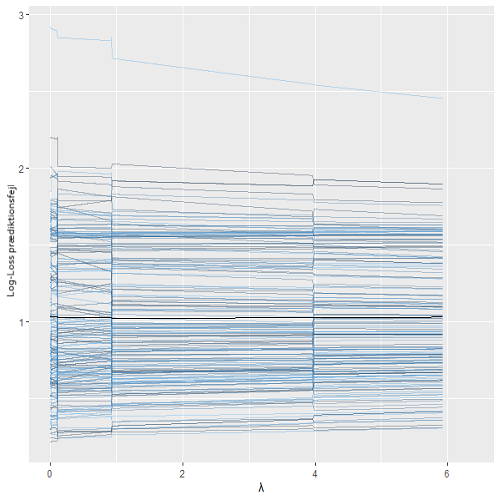
\includegraphics[width=\textwidth]{LOGLOSSSTATISK1.png}
    \caption{Log-prædiktionsfejl mod $\lambda$ for den Generelle Rao Kupper model med lasso-straf, hvor hver linje viser fejlene tilhørende én kamp, og den sorte linje viser gennemsnittet af fejlene}
    \label{fig:LogLossStat}  
    \end{subfigure}
  \begin{subfigure}[b]{0.4\textwidth}
    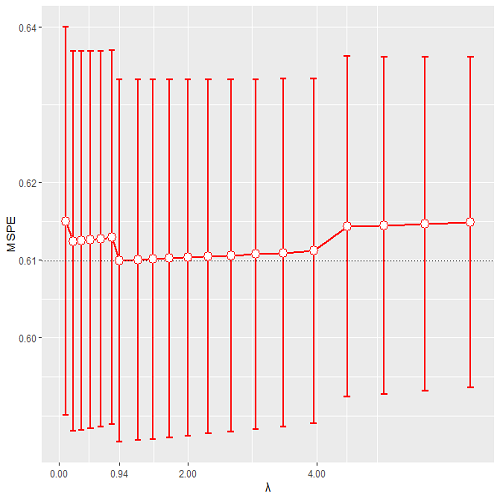
\includegraphics[width=\textwidth]{MSPEBARPLOTSTATNY1.png}
    \caption{Zoomet ind på den sorte linje i ovenstående figur, viser altså MSPE for hver $\lambda$. Hver ende på barene viser en standardfejl for MSPE'en fra Rao Kupper modellen med lasso-straf                                       }
    \label{fig:MSPEBarStat}
  \end{subfigure}
      \hspace{0.2cm}
    \begin{subfigure}[b]{0.4\textwidth}
    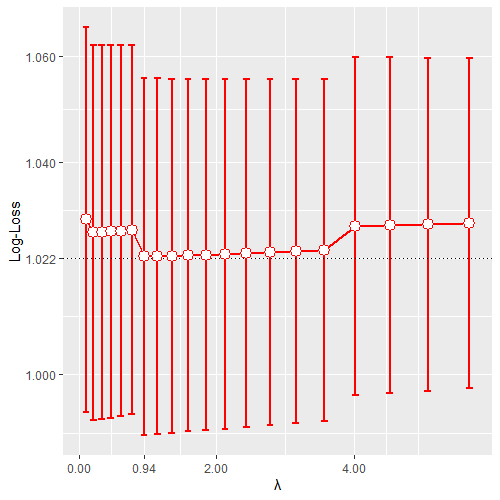
\includegraphics[width=\textwidth]{STATLOGLOSSBARNY1.png}
    \caption{Zoomet ind på den røde linje i ovenstående figur, viser altså gennemsnitlig Log-Loss for hver $\lambda$. Hver ende på barene er en standardfejl fra gennemsnittet for Rao Kupper Modellen med lasso-straf}
    \label{fig:LogLossBarStat}  
    \end{subfigure}
\caption{\textit{MSPE og Log-Loss fra Kryds-Validering i Rao Kupper Modellen}}
\label{fig:MSPELOGLOSSStatisk}
\end{figure}
\begin{table}[ht]
\centering
\begin{adjustbox}{max width=\textwidth}
\begin{tabular}{|l|cc|}
\hline 
 & MSPE & Log-Loss  \\
 \hline
Baseline & 0.639 & 1.057 \\
Rao Kupper & 0.615 & 1.028 \\
Dynamisk & 0.6e6 & 1.064 \\
Rao Kupper Lasso ($\lambda=0.94$)& 0.611 & 1.022 \\
Dynamisk Lasso ($\lambda=3$) & 0.607 & 1.018 \\
   \hline   
\end{tabular} 
\end{adjustbox}
\caption{\label{tab:KVMSPELOGLOSS}\textit{Prædiktionsfejl for de to modeller med og uden lasso-straf, samt prædiktionsfejl for Baseline, som er lavet ud fra den konstante prædiktion $(\bar{Y}_{i \cdot ij},\bar{Y}_{j \cdot ij}, \bar{Y}_{0 \cdot ij)} = (0.456,0.322,0.222)$}}
\end{table}
\newpage
Tabel \ref{tab:EstKoefOptLambda} viser de estimerede koefficienter tilhørende Rao Kupper Modellen og den Dynamiske Model hvor $\lambda$ er henholdsvis $0.94$ og $3$. I Rao Kupper Modellen er der fire aktive parametre, og i den Dynamiske Model er der syv. Standardfejlene er ikke blevet meget mindre, end de var før lasso-straffen, og vi kan dermed ikke konkludere noget nyt i forhold til deres signifikans.\\
\newpage
For at kunne evaluere hvordan de to modeller præsterer med lasso-straffen på ukendt data, har vi valgt at teste dem på Superligaen for sæson 2014-2015, hvor vi starter fra 3. runde. Vi måler dem igen op i mod hinanden med MSPE og Log-Loss prædiktionsfejl, og har yderligere tilføjet \textit{Odds-Fejl}. Odds-Fejl bruger vi som et benchmark for hvordan vores modellers prædiktioner måler sig op imod de odds Bookmakerne har sat på kampene. De odds vi måler op imod er gennemsnitlige odds fra diverse Bookmakere og er hentet fra Oddsportal.com. Vi skriver $odds_i(t),\; odds_j(t), \; odds_0(t)$ som henholdsvis odds for hjemmesejr, odds for udesejr og odds for uafgjort tilhørende kampen $t$. Hvor $t \in \{13,...,198 \}$ repræsenterer hvilken kamp vi er i, bliver Odds-Fejlen udregnet ved:\\
\begin{align*}
    Odds-Fejl &= \sum_t \hat{p}_{i\cdot ij}(t)odds_i(t)+\hat{p}_{j\cdot ij}(t)odds_j(t)+\hat{p}_{0\cdot ij}(t)odds_0(t) -1
\end{align*}
Denne fejl kan symboliseres ved at man ved hver kamp har en omkostning på $1$ og indtjening på $\hat{p}_{i\cdot ij}(t)odds_i(t)+\hat{p}_{j\cdot ij}(t)odds_j(t)+\hat{p}_{0\cdot ij}(t)odds_0(t)$, dermed bliver omkostningen fordelt på de forskellige udfald ud fra de tilhørende sandsynligheder, hvorefter den samlede profit/tab vil være Odds-fejlen. 
\begin{table}[ht!]
\centering
\begin{adjustbox}{max width=\textwidth}
\begin{tabular}{|l|cc|cc|}
\hline
\multicolumn{1}{|l|}{} & \multicolumn{2}{l|}{Rao Kupper Model} & \multicolumn{2}{l|}{Dynamisk Model} \\\hline 
Parameter & Estimeret Koefficient & SE & Estimeret Koefficient & SE\\
 \hline
HjemmeBaneFordel & - & - & 0.139 & 0.071\\
SejrStreak & - & - & -0.150 & 0.105 \\
FifaRating & - & - & 0.230 & 0.150 \\
Hjørne & - & - & 0.150 & 0.130 \\
OffSide  & - & - & -0.037 & 0.122 \\
MålScoret  & 0.224 & 0.196 & 0.170 & 0.141 \\
MålLukketInd  & -0.380 & 0.162 & - & -\\
Tilskuere & 0.061 & 0.134 & - & -\\
BoldBesiddelse & - & - & -0.062 & 0.123  \\
Skud & - & - & - & -\\
SkudIndenfor & - & - & - & -\\
Frispark & -0.005 & 0.130 & - & -\\
$\theta$ & 1.662 & 0.120 & 1.641 & 0.118\\
   \hline   
\end{tabular} 
\end{adjustbox}
\caption{\label{tab:EstKoefOptLambda}\textit{Estimerede parameter koefficienter for de to modeller med deres optimale $\lambda$-værdier fundet ved MSPE og Log-Loss prædiktionsfejl}}
\end{table}\\
\begin{table}[hbt!]
\centering
\begin{adjustbox}{max width=\textwidth}
\begin{tabular}{|l|ccc|}
\hline 
Model & MSPE & Log-Loss & Odds-Fejl \\
 \hline
Rao Kupper Model & 0.618 & 1.030 & -0.035\\
Dynamisk Model & 0.590 & 0.993 & -0.015 \\
   \hline   
\end{tabular} 
\end{adjustbox}
\caption{\label{tab:MSPELOGLOSODDSFEJL}\textit{Prædiktionsfejlene for Rao Kupper modellen og den Dynamiske model med de estimerede koefficienterne fra Table (\ref{tab:EstKoefOptLambda}).}}
\end{table}\\

\clearpage
\section{Diskussion}
Tabel \ref{tab:EstKoefOptLambda} viser de endelige estimater for parameterkoefficienterne tilhørende Rao Kupper modellen og den Dynamiske Model. Til at estimere koefficienterne til den Dynamiske model valgte vi at bruge $\alpha=3$, eftersom den gav den største likelihoodværdi i vores insample test. Eftersom vi har valgt $\alpha$-værdien ved blot at fitte modellen på det fulde data, har vi ikke noget belæg for at den valgte værdi vil passe godt på ukendt data. En anden og måske bedre metode til at vælge denne $\alpha$-værdi ville være at udvælge den ved krydsvalidering, på samme vis som vi har valgt $\lambda$-værdien, ydermere kunne der testes på flere års data, for at få et mere generelt billede af hvordan den influerer på modellen. I det hele taget ville det være mere relevant at estimere den Dynamiske models parametre ud fra flere års data, især når den skal bruges til at prædiktere på ukendt data. Det samme gælder Rao Kupper modellen, hvis man gerne vil få et indblik i hvilke kovariater der influerer på rangeringen. Hvis det eneste der ønskes med Rao Kupper modellen er at rangere nogle hold eller produkter, kan man med fordel estimere styrkerne direkte uden brug af data, ud fra ligning (\ref{func:LikelihoodUdenBeta}). \textcolor{blue}{Ved at estimere styrkerne ved den metode, vil man også mindske risikoen for Type I og II fejl, eftersom der vil være færre parametre at teste.} \\


\textbf{produktsammenligning}
\section{Konklusion}
Konklusion
\clearpage
\section{Litteraturliste}
Litteraturliste
\clearpage
\section{Appendiks}

\printbibliography %Printer referencer

\end{document}